\documentclass{book}
% comment out the following line if you want to latex the whole book:
%\includeonly{ch9}
  % preamble

\usepackage{verbatim}\usepackage{epsf}

\setlength{\textwidth}{5.2in}            % default seems to be around 4.8 inch,
\addtolength{\evensidemargin}{-0.2in}    % so we can devide the extra 0.4 inch
\addtolength{\oddsidemargin}{-0.2in}     % equally over left and right margin

\setlength{\parindent}{2.5em}
\setlength{\parskip}{1.2 ex plus0.2ex minus 0.1ex}
\renewcommand{\baselinestretch}{1.05}
\renewcommand{\floatpagefraction}{1.0}
\renewcommand{\topfraction}{1.0}

\begin{document}
  \frontmatter
\makebox[3.5in][s]{}\verb=Time-stamp: <2002-05-14 13:16:39 piet>=
%
% nice latex feature: you can specify which files you want to include in your
% next output, by listing only those files as arguments to \includeonly{} 
% above on the third line (I had to put this comment here, since the emacs
% time stamp is only recognized in the first eight lines).
% NOTE: if you want to print out the whole book, simply comment out the line
% starting with \includeonly above.
%
% It is a good idea to write this top level file out, each time a change has
% been made, in order to get the correct time stamp to appear on the title
% page.  Even if you print out only one chapter, still the title page will
% appear, so that the time stamp will be include (otherwise the time stamp
% would appear uselessly on a separate white page, before the chapter).
%
    \def\half{{\ifmmode{{1 \over 2}}\else{${1 \over 2}$}\fi}}
\def\dhalf{{\textstyle {1 \over 2}}}
\def\threehalf{{\ifmmode{{3 \over 2}}\else{${3 \over 2}$}\fi}}
\def\dthreehalf{{\textstyle {3 \over 2}}}
\def\dfivehalf{{\textstyle {5 \over 2}}}
\def\dfivethree{{\textstyle {5 \over 3}}}
\def\bx{{\bf x}}
\def\br{{\bf r}}
\def\bv{{\bf v}}
\def\ba{{\bf a}}
\def\bj{{\bf j}}
\def\bs{{\bf s}}
\def\bc{{\bf c}}
\def\bp{{\bf p}}
\def\bk{{\bf k}}
\def\badot{{\bf \dot a}}
\def\batwo{{{\bf  a}^{(2)}}}
\def\bathree{{{\bf  a}^{(3)}}}
\def\bR{{\bf R}}
\def\bV{{\bf V}}
           % input, not include, since all files need the \def{}
    % title page

\thispagestyle{empty}                 % suppresses page numbering of first page

\begin{latexonly}

\begin{center}


\hbox{}

\bigskip\bigskip


{\lggggb Moving Stars Around}

\bigskip


\bigskip\bigskip


{\lggb A Preliminary Version}


\medskip


{\lggb of what will expand into}


\medskip

{\lggb Volumes 1,2,3}

\medskip

{\lggb of the series}

\bigskip\bigskip

{\lgggb The Art of Computational Science}

\bigskip\bigskip

\end{center}

\end{latexonly}


\begin{htmlonly}


\begin{center}


\hbox{}

\bigskip\bigskip


{\huge \bf Moving Stars Around}

\medskip


{\LARGE A Preliminary Version}



{\LARGE of what will expand into}


\medskip



{\LARGE Volumes 1,2,3}

\medskip



{\LARGE of the series}


\bigskip


{\huge \bf The Art of Computational Science}



\bigskip


\end{center}
\end{htmlonly}

 \begin{latexonly}
 \begin{center}
 \leavevmode
 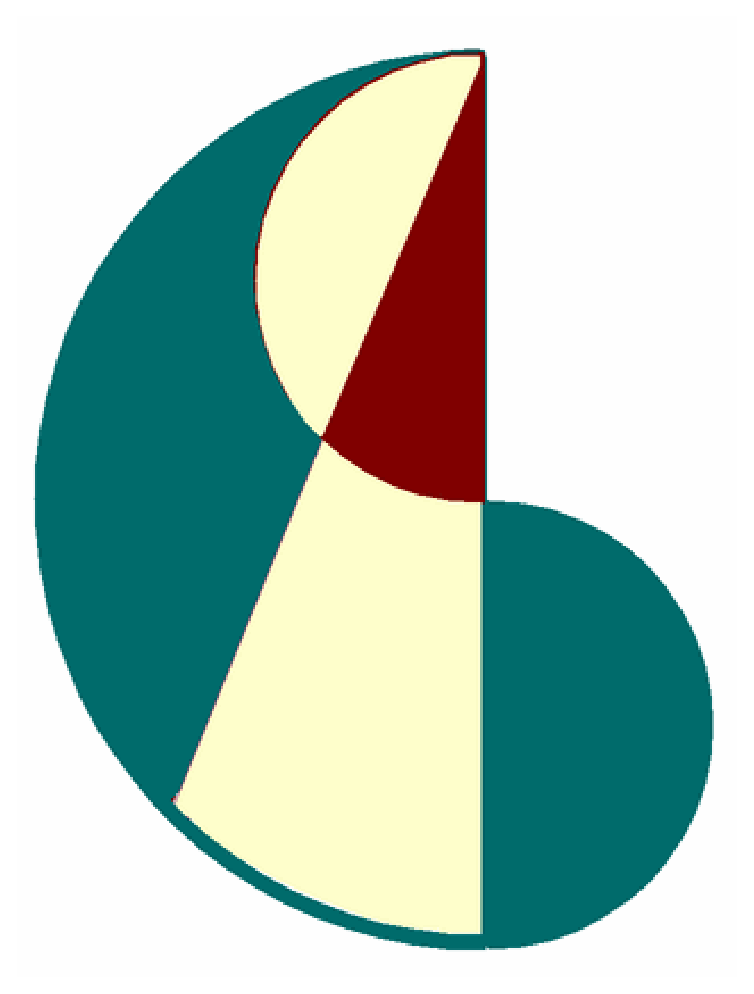
\includegraphics[width=4cm]{acstitle.eps}
 \end{center}
 \end{latexonly}


\begin{htmlonly}
\begin{center}
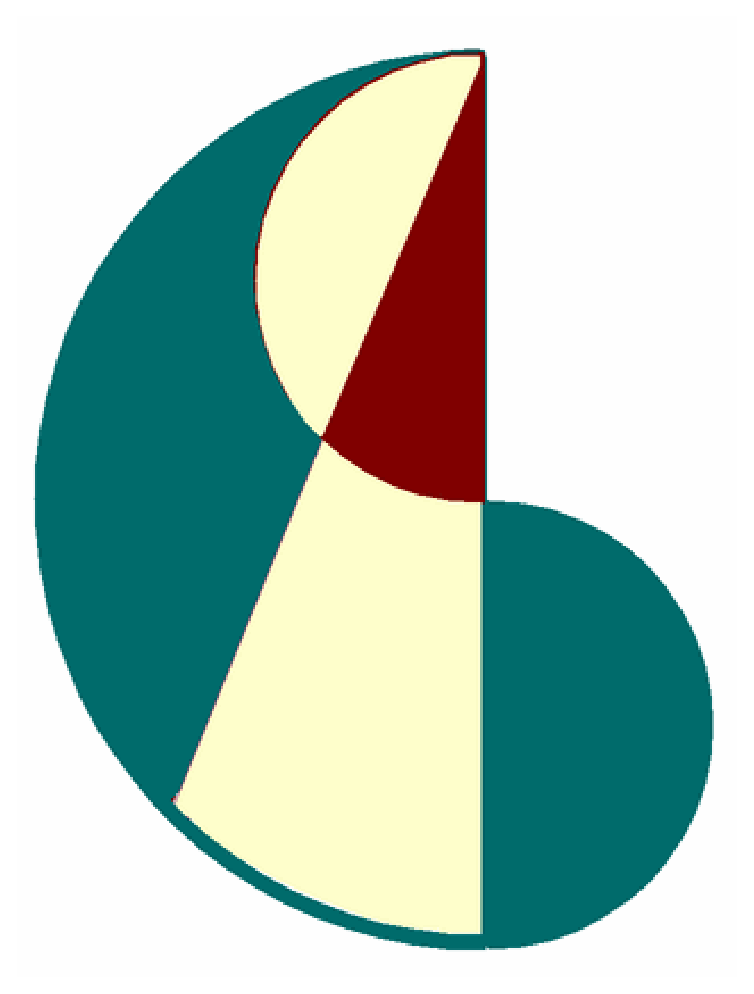
\includegraphics[width=3cm]{acstitle.eps}
\end{center}
\end{htmlonly}

\bigskip\bigskip\bigskip


\begin{center}
% lggr -> Large
% lr -> large
\begin{tabular}{llllllll}
& {\LARGE Piet Hut} & {\LARGE \&} & & & & & {\LARGE Jun Makino}\\
&  & & & & & & \\
& {\large Institute for Advanced Study} & & & & & &
  {\large Univ. of Tokyo, \ Dept. of Astronomy}\\
& {\large 1 Einstein Drive} & & & & & & {\large 7-3-1 Hongo, Bunkyo-ku}\\
& {\large Princeton, NJ 08540} & & & & & & {\large Tokyo 113-0033}\\
& {\large U.S.A.} & & & & & & {\large JAPAN}\\
& {\large piet@ias.edu} & & & & & & {\large makino@astron.s.u-tokyo.ac.jp}\\
\end{tabular}

\bigskip\bigskip\bigskip\bigskip

\end{center}
         % input, in order to let the time stamp appear
%
% uncomment the following three lines, if you want to print two pages
% on one, using e.g. "psnup -2 v1.ps > v1_2.ps".  Normally the next three
% lines should be commented out, but in that case psnup will print the right
% (left) pages on the left (right) side.
%
%\newpage
%\thispagestyle{empty}
%\mbox{}
%
    \newpage           % blank page, to force preface to start on a right hand page
\thispagestyle{empty}      % suppresses page numbering of the blank second page
\mbox{}                    % dummy content; otherwise \newpage has no effect
\newpage                   % on to third page, to start the preface
\pagenumbering{roman}      % with a roman numbering system, starting here at i

%%\chapter{Preface} %% this replace the four lines below, but at the
                    %% cost (currently) of two extra pages

\addcontentsline{toc}{chapter}{Preface}

\begin{center}
{\lgb Preface}
\end{center}

The {\it Pure Gravity} book series, of which this is the second volume,
\dots\dots\dots

%\bigskip
%\bigskip
%{\it Acknowledgments:}
%xxx
%We thank xxx, xxx and xxx for valuable
%discussions.  This work is supported in part by the Research for the
%Future Program of Japan Society for the Promotion of Science
%(JSPS-RFTP97P01102).

\tableofcontents

\listoffigures


  \mainmatter
      \chapter{The Universe in a Computer}

\section{Gravity}

Gravity is the weakest of all fundamental forces in physics, far
weaker than electromagnetism or the so-called weak and strong
interactions between subatomic particles.  However, the other three
forces lose out in the competition with gravity over long distances.
The weak and strong interactions both have an intrinsically short
range.  Electromagnetism, while being long-range like gravity, suffers
from a cancellation of attraction and repulsion in bulk matter, since
there tend to be as almost exactly as many positive as negative
charges in any sizable piece of matter.  In contrast, gravitational
interactions between particles are always attractive.  Therefore, the
larger a piece of matter is, the more gravitational force it exerts on
its surroundings.

This dominance of gravity at long distances makes the job of
modeling a chunk of the Universe easier.  To a first approximation, it
is often a good idea to neglect the other forces, and to model the
objects as if they were interacting only through gravity.  In many
cases, we can also neglect the intrinsic dimensions of the objects,
treating each object as a point in space with a given mass.  All this
greatly simplifies the mathematical treatment of a system, by leaving
out most of the physics and chemistry that would be needed in a more
accurate treatment.

This book is the first in a series of books titled {\it Pure Gravity}, to
indicate that we are making this approximation of treating objects as
gravitating masses and nothing more.  The objects we will be studying
are stars, and the environment we will focus on are dense stellar
systems, where the stars are so close together that they will
occasional collide and in general have frequent interesting and
complex interactions.  In a later series, {\it Applied Gravity}, we will
look at the internal physics of those stars: how they evolve under the
influence of nuclear reactions in their centers, how they may die in
cosmic explosions, and what happens to their remnant cores.  We will
especially study how interactions between stars of all types can change
their evolutionary behavior through two-body, three-body, and more
complex interactions, leading to an intricate `star cluster ecology'.

This first book, {\it Writing an N-Body Code}, lays the groundwork for
modeling a system of stars.  We start absolutely from scratch, with a
most simple code of less than a page long.  In many small steps we
then improve that code, pointing out the many pitfalls along the way,
on the level of programming as well as astrophysical understanding.
We introduce helpful code development facilities and give many hints as
to how to balance simplicity, efficiency, clarity, and modularity of
the code.  Our intention is to introduce the topic from square one,
and then to work our way up to a robust set of codes with which one
can do actual research.  In later volumes in this series, we will
continue to develop these codes, adding many useful diagnostic tools,
and integrating those in a full production-level software environment.

\section{Galactic Suburbia}

The sun is a star like any other among the hundred billion or so stars
in our galaxy.  It is unremarkable in its properties.  Its mass is in
the mid range of what is normal for stars: there are others more than
ten times more massive, and there are also stars more ten times less
massive, but the vast majority of stars have a mass within a factor
ten of that of the sun.  Our home star is also unremarkable in its
location, at a distance of some thirty thousand light years from the
center of the galaxy.  Again, the number of stars closer to the center
and further away from the center are comparable.  Our closest neighbor,
Proxima Centauri, lies at a distance of a bit more than four light years.

This distance is typical for separations between stars in our neck of
the woods.  A light year is ten million times larger than the diameter
of the sun (a million km, or three light seconds).  In a scale model,
if we would represent each star as a cherry, an inch across, the
separation between the stars would be many hundreds of miles.  It is
clear from these numbers that collisions between stars in the solar
neighborhood must be very rare.  Although the stars follow random
orbits without any traffic control, they present such tiny targets
that we have to wait very long indeed in order to witness two of them
crashing into each other.  A quick estimate tells us that the sun has
a chance of hitting another star of less than $10^{-18}$ per year.  In
other words, we would have to wait at least $10^{18}$ years to have an
appreciable chance to witness such a collision.  Given that the sun is
less than five billion years old, it is no surprise that it does not
show any signs of a past collision: the chance that that would have
happened was less than one in a hundred million.  Life in our galactic
suburbs is really quite safe for a star.

There are other places in our galaxy that are far more crowded, and
consequently are a lot more dangerous to venture into.  We will have
a brief look at four types of crowded neighborhoods.

\section{Globular Clusters}

\begin{figure}[ht]
\centering
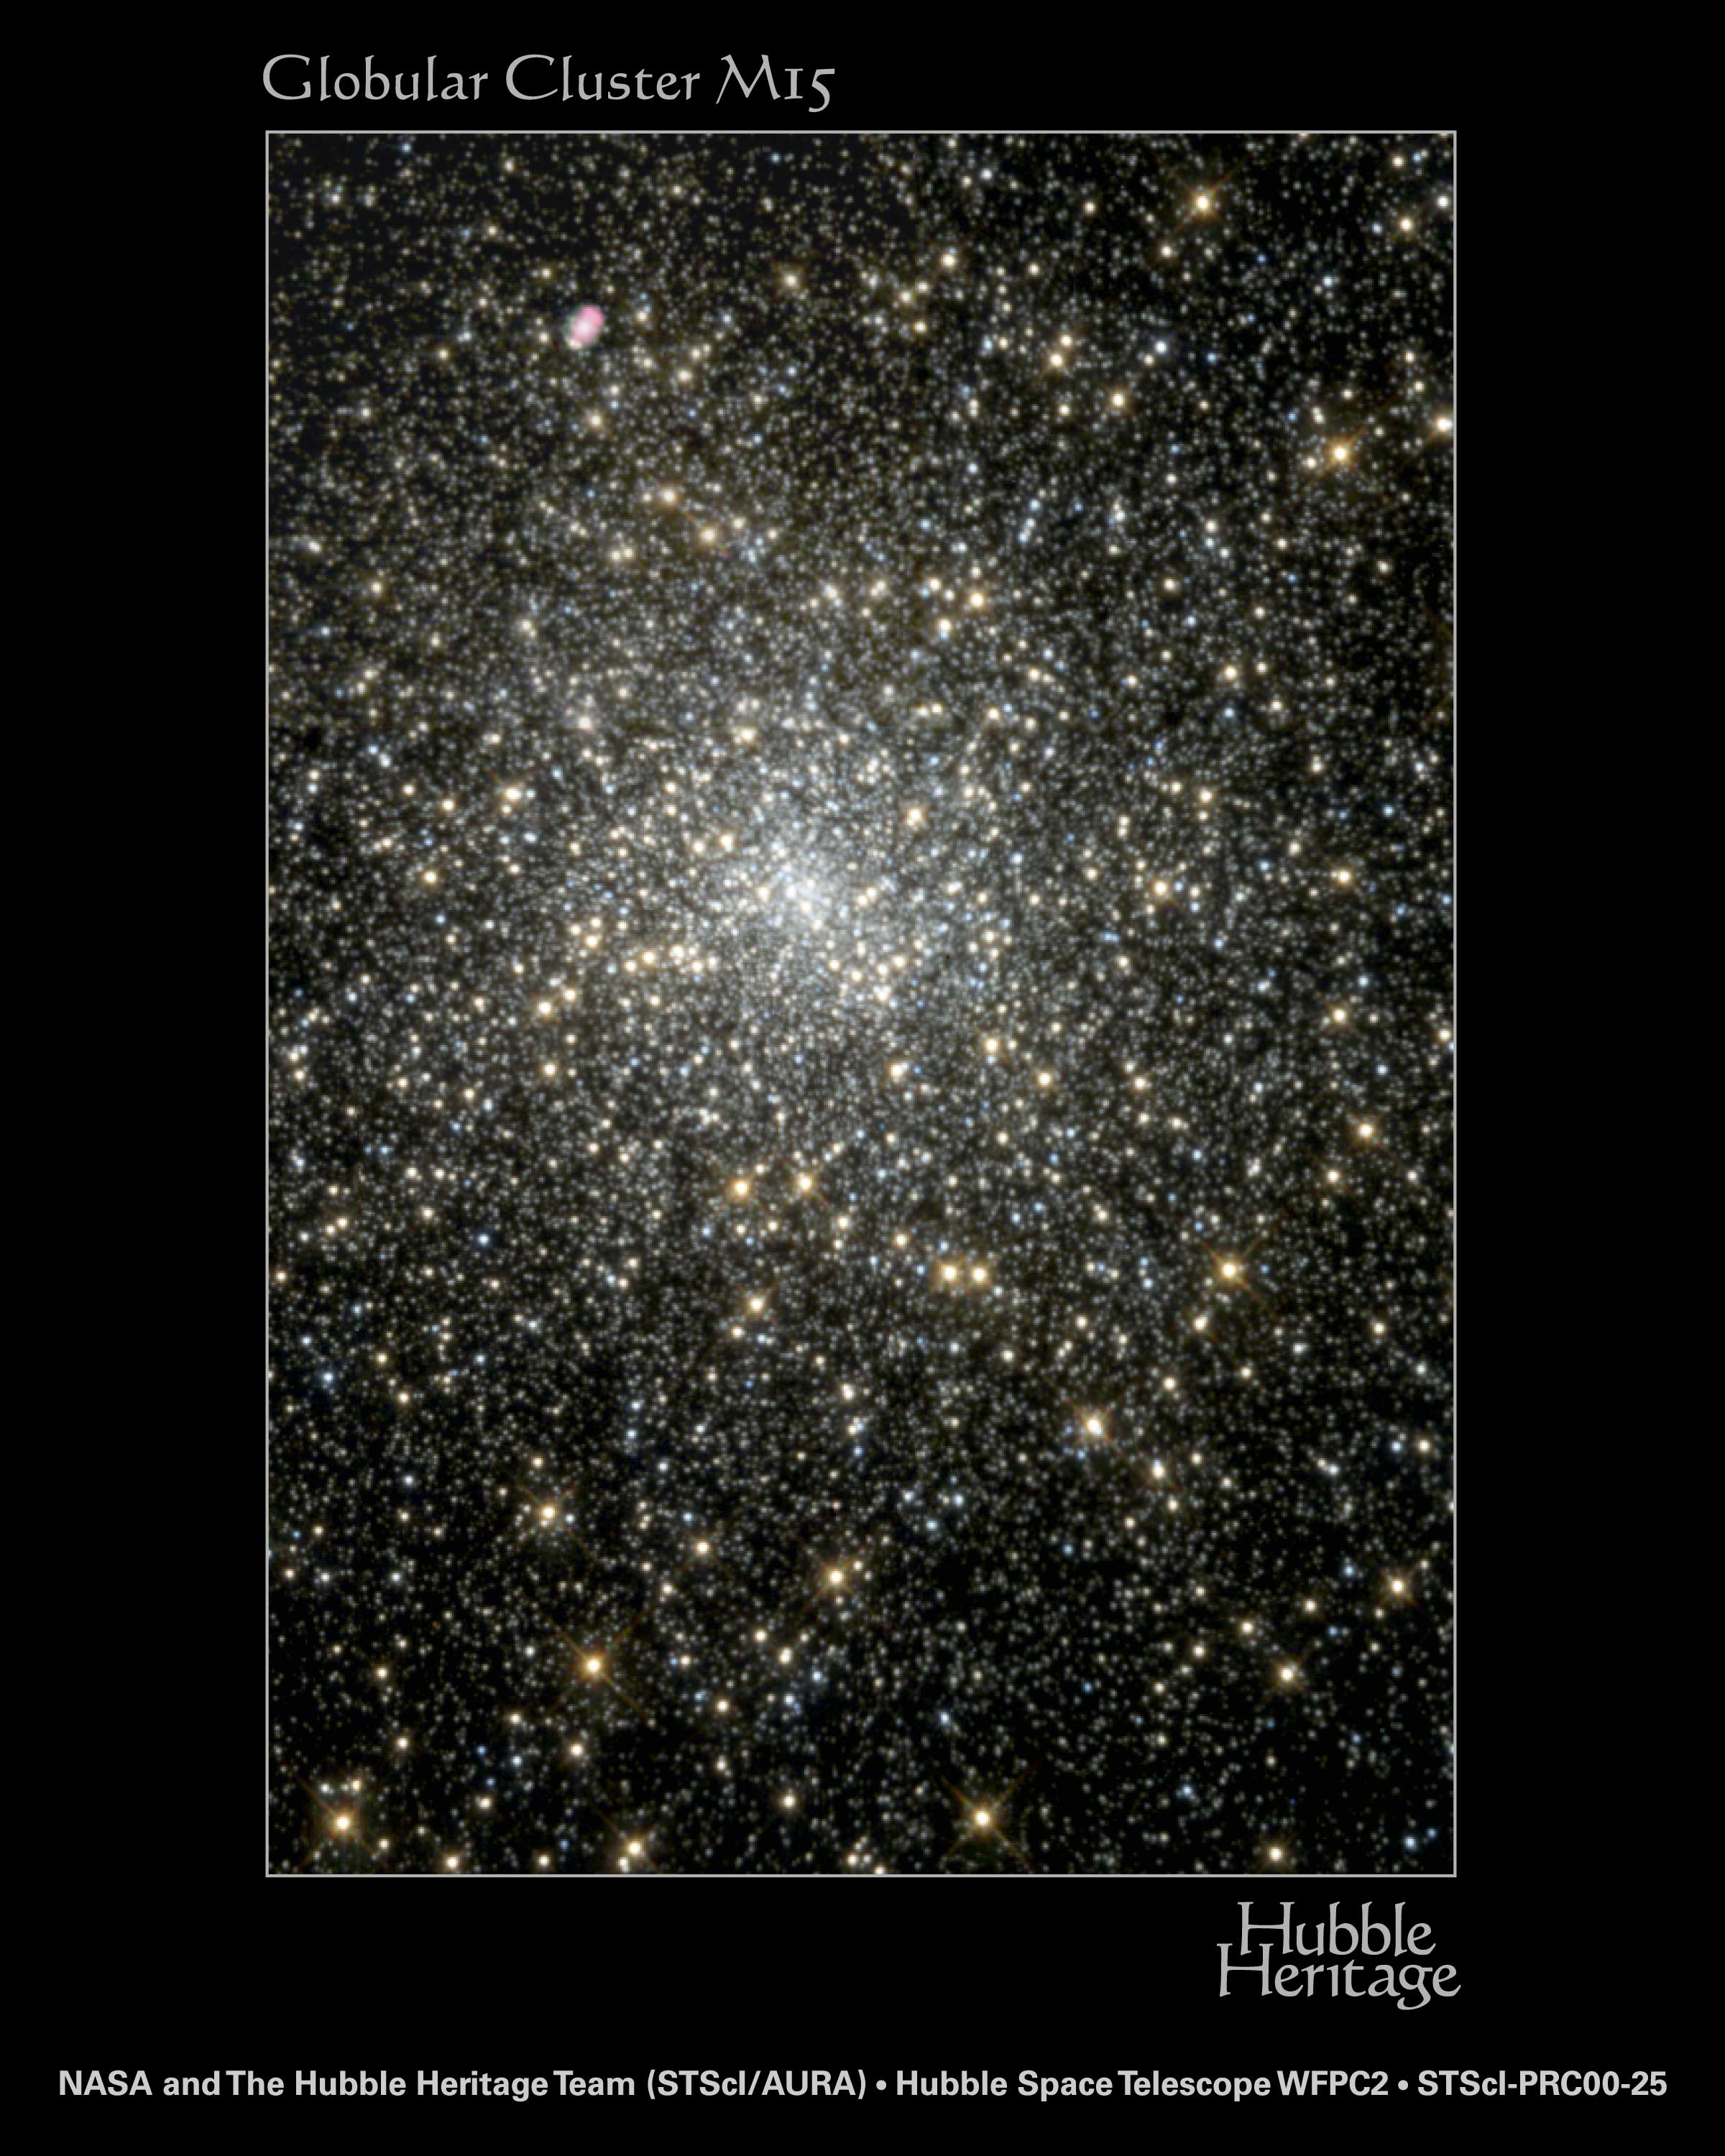
\includegraphics[width=4.5in]{chap1/m15.eps}
\caption[A snapshot of the globular cluster M15]
{A snapshot of the globular cluster M15, taken with the Hubble Space
Telescope.}
\label{fig:m15}
\end{figure}
%%  From: http://oposite.stsci.edu/pubinfo/PR/2000/25/content/0025y.jpg

In Fig. \ref{fig:m15} we see a picture of the globular cluster M15,
taken with the Hubble Space Telescope.  This cluster contains roughly
a million stars.  In the central region typical distances between
neighboring stars are only a few hundredth of a light year, more than
a hundred times smaller than those in the solar neighborhood.  This
implies a stellar density that is more than a million times larger
than that near the sun.  Since the typical relative velocities of
stars in M15 are comparable to that of the sun and its neighbors, a
few tens of km/sec, collision times scale with the density, leading to
a central time between collisions of less than $10^{12}$ years.  With
globular clusters having an age of more than $10^{10}$ years, a typical
star near the center already has a chance of more than a percent to
have undergone a collision in the past.  

In fact, the chances are much higher than this rough estimate indicates.
One reason is the stars spend some part of their life time in a much
more extended state.  A star like the sun increases its diameter by
more than a factor of one hundred toward the end of its life, when
they become a red giant.  By presenting a much larger target to other
stars, they increase their chance for a collision during this stage
(even though this increase is partly offset by the fact that the red
giant stage lasts shorter than the so-called main-sequence life time
of a star, during which they have a normal appearance and diameter).
The other reason is that many stars are part of a double star system,
a type of dynamic spider web that can catch a third star, or another
double star, into a temporary three- or four-body dance.  Once engaged
in such a dance, the local stellar crowding is enormously enhanced,
and the chance for collisions is greatly increased. 

A detailed analysis of all these factors predicts that a significant
fraction of stars in the core of a dense globular cluster such as M15
has already undergone at least one collision in its life time.  This
analysis, however, is quiet complex.  To study all of the important
channels through which collisions may occur, we have to analyze
encounters between a great variety of single and double stars, and
occasional bound triples and larger bound multiples of stars.  Since
each star in a bound subsystem can be a normal main-sequence star, a
red giant, a white dwarf, a neutron star or even a black hole, as well
as an exotic collision product itself, the combinatorial richness of
flavors of double stars and triples is enormous.  If we want to pick a
particular double star, we not only have to choose a star type for
each of its members, but in addition we have to specify the mass of
each star, and the parameters of its orbit, such as the semimajor axis
(a measure for the typical separation of the two stars) as well as the
orbital eccentricity.

The goal of our book series is to develop the software tools to make
it possible to simulate an entire star cluster like M15, and to
analyze the resulting behavior both locally and globally.

\clearpage  % to let the m15 picture be inserted not further than here

\section{Galactic Nuclei}

In Fig. \ref{fig:gc} we see an image of the very center of our galaxy.
This picture is taken with the Northern branch of the two Gemini
telescopes, which is located in Hawaii on top of the mountain Mauna Kea.

\begin{figure}[ht]
\centering
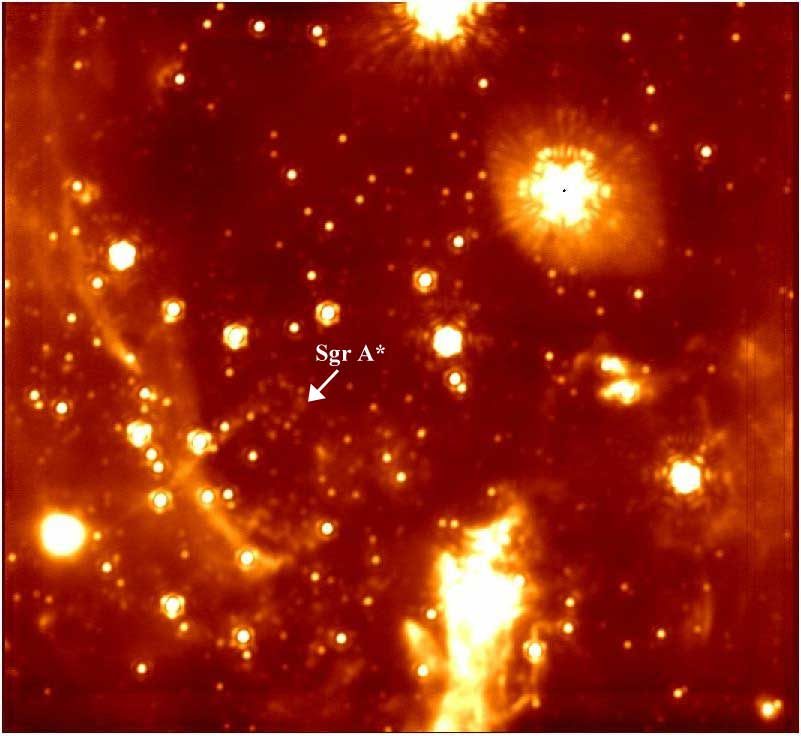
\includegraphics[width=4.5in]{chap1/gc.eps}
\caption[An image of the central region of our galaxy]
{An image of the central region of our galaxy, taken with the Gemini
North telescope.  The center is located on the right just above the
bottom edge of the image.}
\label{fig:gc}
\end{figure}
%% From: http://www.gemini.edu/gallery/observing/gc\_color.jpg

In the very center of our galaxy, a black hole resides with a mass
a few million times larger than the mass of our sun.  Although the
black hole itself is invisible, we can infer its presence by its
strong gravitational field, which in turn is reflected in the speed
with which stars pass near the black hole.  In normal visible light it
is impossible to get a glimpse of the galactic center, because of the
obscuring gas clouds that are positioned between us and the center.
Infrared light, however, can penetrate deeper in dusty regions.
Fig. \ref{fig:gc} is a false-color image, reconstructed from
observations in different infrared wavelength bands.

In the central few light years near the black hole, the total mass of
stars is comparable to the mass of the hole.  This region is also
called the galactic nucleus.  Here the stellar density is at least as
large as that in the center of the densest globular clusters.  However,
due to the strong attraction of the black hole, the stars zip around at
much higher velocities.  Whereas a typical star in the core of M15 has
a speed of a few tens of km/sec, stars near the black hole in the
center of our galaxy move with speeds exceeding a 1000 km/sec.  As a
consequence, the frequency of stellar collisions is strongly enhanced.

Modeling the detailed behavior of stars in this region remains a great
challenge, partly because of the complicated environmental features.
A globular cluster forms a theorist's dream of a laboratory, with its
absence of gas and dust and starforming regions.  All we find there
are stars that can be modeled well as point particles unless they come
close and collide, after which we can apply the point particle
approximation once again.  In contrast, there are giant molecular
clouds containing enormous amounts of gas and dust right close up to
the galactic center.  In these clouds, new stars are formed, some of
which will soon afterwards end their life in brilliant supernova
explosions, while spewing much of their debris back into the
interstellar medium.  Such complications are not present in globular
clusters, where supernovae no longer occur since the member stars are
too old and small to become a supernova.

Most other galaxies also harbor a massive black hole in their nuclei.
Some of those have a mass of hundreds of millions of solar masses, or
in extreme cases even more than a billion times the mass of the sun.
The holy grail of the study of dense stellar systems is to perform and
analyze accurate simulations of the complex ecology of stars and gas
in the environment of such enormous holes in space.  Much of the
research on globular clusters can be seen as providing the initial
steps toward a detailed modeling of galactic nuclei.

\section{Star Forming Regions}

\begin{figure}[ht]
\centering
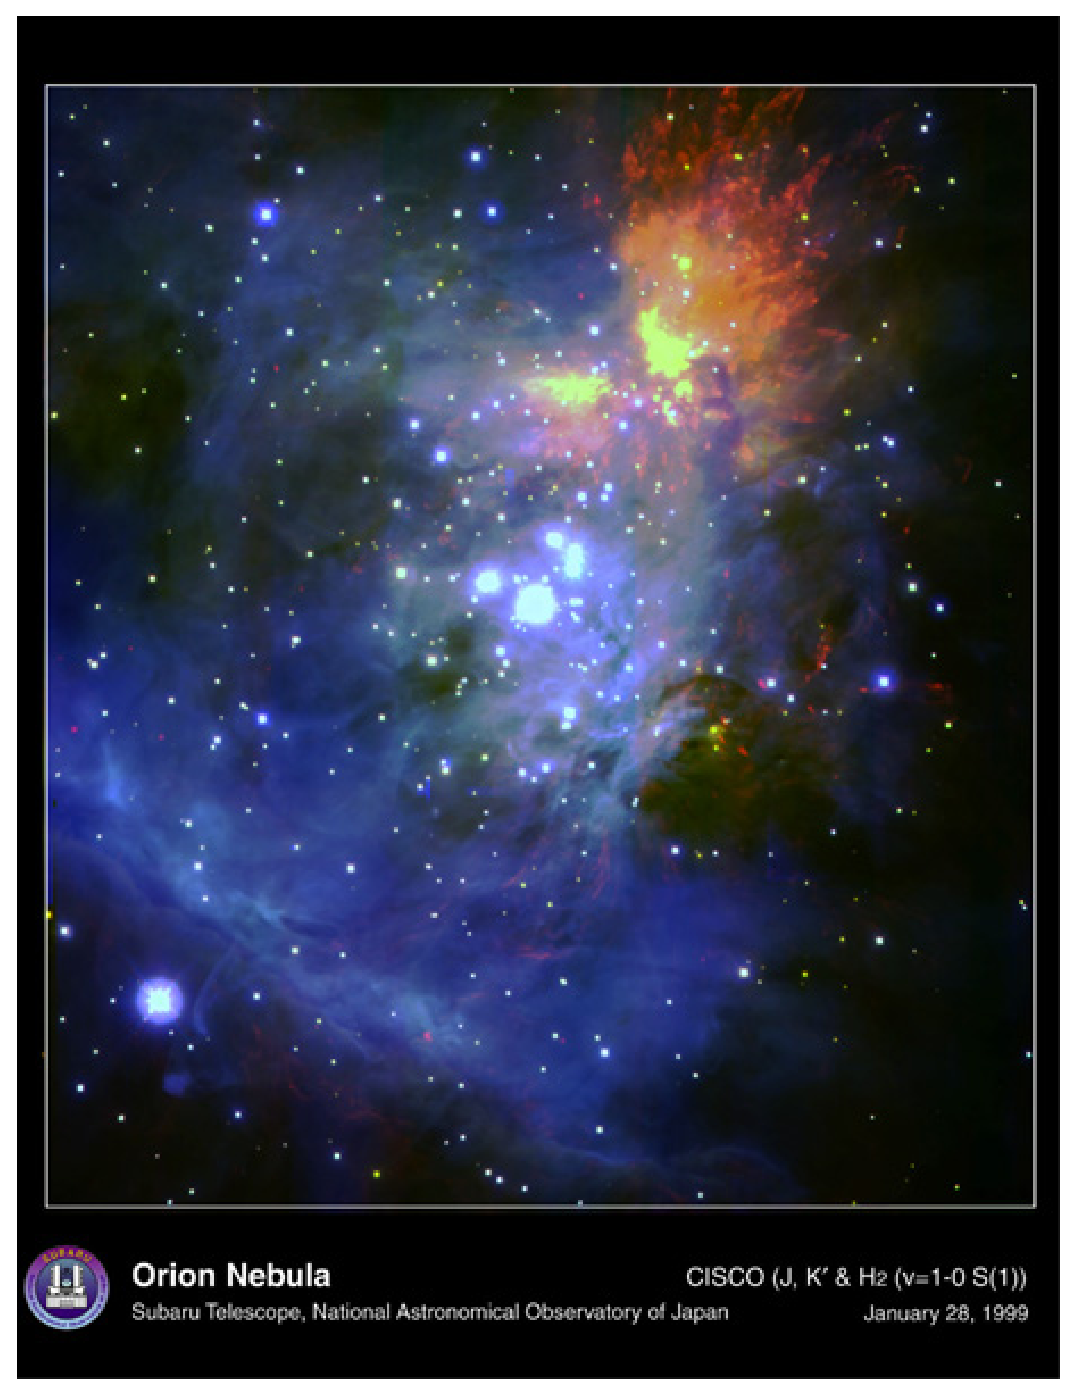
\includegraphics[width=3in]{chap1/orion.eps}
\caption[The Orion Nebula]
{The Orion Nebula, as seen by the Subaru telescope.}
\label{fig:orion}
\end{figure}
%%  From: http://www.subaru.naoj.org/Science/press\_release/9901/Orion.jpg

There are many other places in the galactic disk where the density of
stars is high enough to make collisions likely, at least temporarily.
These are the sites where stars are born.  Fig. \ref{fig:orion} taken
by the Japanese Subaru telescope in Hawaii shows the Orion Nebula,
also known as M42, at a distance of 1500 light years from the sun.
This picture, too, is taking in infrared light in order to penetrate
the dusty regions surrounding the young stars.  The four brightest
stars in the center, collectively known as the Trapezium, form the
most massive stars of a larger conglomeration of stars, all recently
formed from the gas and dust that still surrounds them.

In order to study collisions in these star forming regions, we can no
longer treat the stars are point masses.  Many of the collisions take
place while the stars are still in the process of forming.  While a
protostar is still in the process of contracting from the gas cloud
in which it was born, it presents a larger target for collisions with
other stars.  In addition, a single contracting gas cloud may fission,
giving rise to more than one star at the same time.  In this way, the
correlated appearance of protostars is even more likely to lead to
subsequent collisions.

The proper way to model these processes is to combine gas dynamics and
stellar dynamics.  Much progress has been made recently in this area.
One way to use stellar dynamics in an approximate fashion is to begin
with the output of the gas dynamics codes, which present the positions
and velocities of a group of newly formed stars, and then to follow
and analyze the motions of those stars, including their collisions.

\section{Open Clusters}

Although stars are formed in groups, these groups typically do not
stay together for very long.  Perturbations from other stars and gas
clouds in their vicinity are often enough to break up the fragile
gravitational hold they initial have over each other.  Some of the
more massive groups of newly formed stars, however, are sufficiently
tightly bound to survive their environmental harassment.  They form
the so-called open clusters, where there name indicates that they have
central densities that are typically less than what we see in globular
clusters.

\begin{figure}[ht]
\centering
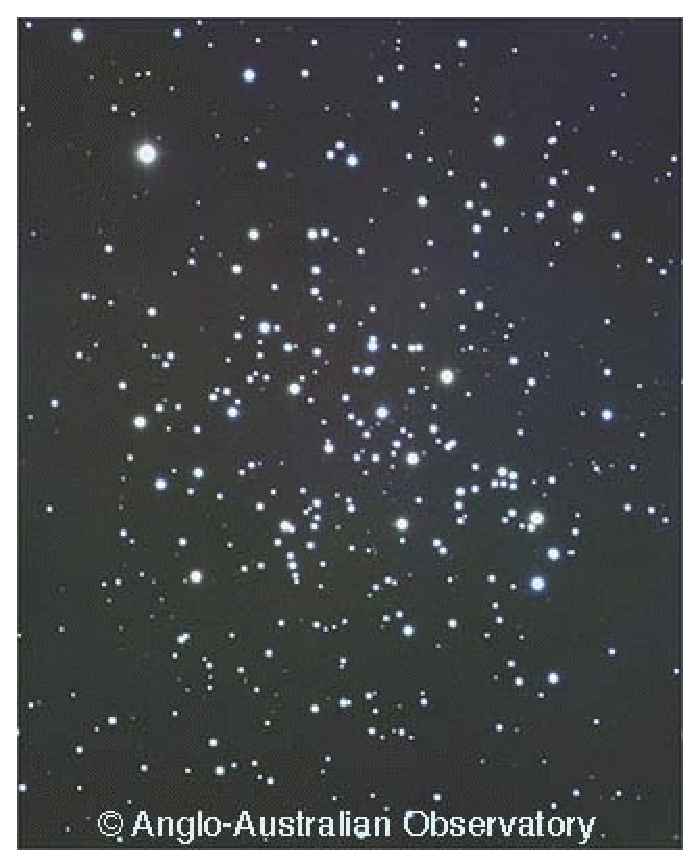
\includegraphics[width=2.5in]{chap1/m67.ps}
\caption[The open star cluster M67]
{The open star cluster M67, in a picture taken by the Anglo-Australian
Observatory.}
\label{fig:m67}
\end{figure}
%%  From: http://www.seds.org/messier/Pics/More/m67aat.jpg

Fig. \ref{fig:m67} shows one of the richest and densest open clusters,
M67, as observed by the Anglo-Australian Observatory.  Since this
cluster is old enough to have lost its gas and dust, all stars are
visible at normal optical wavelengths, at which this image is taken.
In the central regions of this cluster, there are indications that
some of the stars have undergone close encounters or even collisions.
Consequently, this star cluster qualifies as a dense stellar system.

Open clusters typically have fewer members than globular clusters.
Also, they are younger.  Both facts makes it easier to simulate open
clusters than globular clusters.  On the other hand, the densest
globular clusters show a higher frequency and a far richer variety of
stellar collisions, making them a more interesting laboratory.  In
that sense, a dynamical simulation of an open cluster can be seen as
providing preparatory steps toward the modeling of globular clusters,
just as a study of the latter forms a stepping stone toward the
investigation of galactic nuclei.

\section{Writing your own star cluster simulator}

Astronomers have almost half a century of experience in writing
computer codes to simulate dense stellar systems.  The first published
results date back to 1960, and it was in the subsequent decade that it
became clear just how tricky it was to simulate a group of interacting
stars.  The task seems so easy: just integrate Newton's equations of
motion for each star, under the influence of the gravitational pairwise
interactions of all other stars.  Indeed, it is straightforward to
write a simple code to do so, as we will see below.  And as long as
all stars remain fairly well separated from each other, even a simple
code will do a reasonably good job.

In practice, though, even a small group of stars will spontaneously
form one or more double stars.  This was discovered experimentally in
the early sixties.  One way to understand this result, after the fact,
is from an energetic point of view.  When a double star, or binary as they
are generally called, is formed, energy is released.  Since the two stars
in a binary are bound, the potential energy is larger than the kinetic
energy, and the total energy is negative.  When three stars come together
randomly, there is a chance that two of the three are left in a bound
state, while the third one escapes, carrying the excess energy.  Left
by itself, a stellar system will exploit this energy liberation
mechanism by spontaneously forming binaries.

As soon as even one binary appears, a simple code with constant time
steps will either crash or resort to a very slow and inefficient crawl.
The changes in the relative configuration of the two stars occur so
frequent that they can be easily missed.  If they are modeled correctly,
by choosing a tiny time step, the rest of the system will be forced to
slow down, while spending a large and unnecessary amount of computer
time on all the other stars that don't need such fine resolution.  By
the end of the sixties, these problems were overcome by the development
of codes that employed individual time steps.  Stars with close
neighbors were stepped forward in time more frequently than stars at
large, and in this way the computational power was brought to where it
was most needed.

This modification in itself brought gravitational $N$-body codes already
well outside the range of systems that are normally discussed in text
books on numerical integration methods.  The internal book keeping
needed to write a correct and efficient code with individual time
steps is surprisingly large, given the simplicity of the task:
integrate the effect of pairwise attractive inverse square forces.
But this was only a first step toward the development of modern $N$-body
codes.  The presence of tight binaries produced much more of an obstacle,
and throughout the seventies a variety of clever mechanisms were developed
in order to deal with them efficiently.

For one thing, there are problems with round-off.  Two stars in a tight
orbit around each other have almost the same position vector, as seen
from the center of a star cluster, where we normally anchor the global
coordinate system.  And yet it is the separation between the stars
that determines their mutual forces.  When we compute the separation
by subtracting two almost identical spatial vectors, we are asking for
(numerical) trouble.  The solution is to introduce a local coordinate
system whenever two or more stars undergo a close interaction.  This
does away with the round-off problem, but it introduces a host of
administrative complexities, in order to make sure that any arbitrary
configuration of stars is locally presented correctly -- and that the
right thing happens when two or more of such local coordinate patches
encounter each other.  This may not happen often, but one occurrence
in a long run is enough to crash the system if no precautions have
been taken for such a situation to happen.

We can continue the list of tricks that have been invented to allow
every larger and denser systems to be modeled correctly.  Numerical
problems with the singularity in the two-body system have been
overcome by mapping two or more interacting stars from the
three-dimensional Kepler problem to a four-dimensional harmonic
oscillator.  The total force on particles has been split into
different contributions, the first from a near zone of relatively
close neighbors and the second from a far zone of all other particles,
with each partial force being governed with different integration time
steps.  Tree codes have been used to group the contributions of a
number of more and more distant zones together in ever larger chunks,
for efficiency.  Triple stars have received their own special treatment,
especially the marginally stable triples that are sometimes long-lived, 
but continuously changed their inner state due to internal perturbations.
The list goes on.

In this first book, we will introduce a modern integrator, the Hermite
scheme, developed in the 1990s, together with a variable time step
integration scheme, where all stars share a common time step at any
given time.  In subsequent volumes in the series, we will introduce
the other refinements mentioned above.  Our emphasis will be on a
complete explanation of all the steps involved, together with a
discussion of the motivation for those steps.  In the last few
chapters, we will embark on a research project featuring stellar
collisions, in a simple gravity-only approximation.

%%    \part{3-Body Scattering in 1D}
%%      \chapter{Regularization}


%%      \chapter{Setting Up and Analyzing Gravitational Scattering Experiments}


%%      \chapter{A Story-Telling Mechanism}


%%    \part{3-Body Scattering in 2D}
%%      \chapter{Automatization of Laboratory Experiments}


%%      \chapter{Exploring $N = 3$ with a Hermite Algorithm}

Having seen the dramatic improvement that came from switching from the
forward Euler algorithm to the leapfrog, the obvious next step was to
go to yet higher order algorithms.  A quick look in a few books of
numerical methods showed our friends that there was a bewildering
choice of third- and fourth-order methods to choose from.  Alice then
mentioned that her thesis advisor had pointed her to an elegant and
natural generalization of the leapfrog algorithm, by the name of the
Hermite scheme.

\section{A Surprisingly Simple Hermite Scheme}

The most symmetric Hermite version, and the one closest resembling the
leapfrog is this one:

\def\half{{\textstyle\frac{1}{2}}}
\def\quarter{{\textstyle\frac{1}{4}}}
\def\one#1{{\textstyle\frac{1}{#1}}}
\def\three#1{{\textstyle\frac{3}{#1}}}
\def\seven#1{{\textstyle\frac{7}{#1}}}

\begin{eqnarray}
\br_{i+1} & = & \br_i + \half(\bv_i + \bv_{i+1}) dt +
                \one{12}(\ba_i - \ba_{i+1})(dt)^2
                \label{hermite-step1} \\
\bv_{i+1} & = & \bv_i + \half(\ba_i + \ba_{i+1}) dt +
                \one{12}(\bj_i - \bj_{i+1})(dt)^2
                \label{hermite-step2}
\end{eqnarray}

Here $\bj = d\ba/dt$ is the {\it jerk}, the time derivative of the
acceleration, and therefore the third time derivative of position:

\begin{equation}
\bj = \frac{d^3}{dt^3} \br
\end{equation}

The term `jerk' has crept into the literature relatively recently,
probably originally as a pun.  If a car or train changes acceleration
relatively quickly you experience not a smoothly accelerating or
decelerating motion, but instead a rather `jerky' one.

The jerk can be computed through straightforward differentiation of
Newton's gravitational equations, Eq. \ref{newton}:

\begin{equation}
\bj_i =  G \sum_{j=1 \atop j \neq i}^N \,M_j \left[
\frac{\bv_{ji}}{r_{ji}^3} - 3 \frac{(\br_{ji}\cdot\bv_{ji})\br_{ji}}{r_{ji}^5}
\right]\label{newton-jerk}
\end{equation}

\noindent
where $\bv_{ji} = \bv_j - \bv_i$.

As an aside, note that the jerk has one very convenient property.
Although the expression above looks quite a bit more complicated than
Newton's original equations, they can still be evaluated through one
pass over the whole $N$-body system.  This is no longer true for
higher derivatives.  For example, we can obtain the fourth derivative
of the position of particle $i$ (the {\it snap}, see next section) by
differentiating Eq. \ref{newton-jerk}:

\begin{eqnarray}
\frac{d^4}{dt^4}\br_i = G \sum_{j=1 \atop j \neq i}^N \,M_j \Bigg[ &\,&
\!\!\!\!\!\!\!\!\!\! \frac{\ba_{ji}}{r_{ji}^3}
-6 \frac{(\br_{ji}\cdot\bv_{ji})}{r_{ji}^5}\bv_{ji} \nonumber \\
 &\,& \!\!\!\!\!\!\!\! + \left\{ -3\frac{v_{ji}^2}{r_{ji}^5}
-3 \frac{(\br_{ji}\cdot\ba_{ji})}{r_{ji}^5}
+15 \frac{(\br_{ji}\cdot\bv_{ji})^2}{r_{ji}^7} \right\} \br_{ji} \,\,\Bigg]
\label{newton-snap}
\end{eqnarray}

\noindent
where $\ba_{ji} = \ba_j - \ba_i$, and this is the expression that
thickens the plot.  Unlike the $\br_{ji}$ and $\bv_{ji}$ expressions,
that are given by the initial conditions, $\ba_{ji}$ has to be
calculated from the positions and velocities.  However, this
calculation does not only involve the pairwise attraction of particle
$j$ on particle $i$, but in fact all pairwise attractions of all
particles on each other!  This follows immediately when we write out
what the shorthand implies:

\begin{equation}
\ba_{ji} = \ba_j - \ba_i = G \sum_{k=1 \atop k \neq j}^N
\frac{M_k}{r_{kj}^3} \,\br_{kj} -  G \sum_{k=1 \atop k \neq i}^N
\frac{M_k}{r_{ki}^3} \,\br_{ki}
\end{equation}

\noindent
When we substitute this back into Eq. \ref{newton-snap}, we see that
we have to do a double pass over the $N$-body system, summing over
both indices $k$ and $j$ in order to compute a single fourth derivative
for the position of particle $i$.  

\section{Comparison with the Leapfrog}

When we look at Eqs. \ref{hermite-step1}, \ref{hermite-step2}, we see
some familiar features.  Neglecting the higher-order term for the
moment, we recognize the leapfrog: the new position is effectively
determined by the mid-point velocity $v_{i+1/2}$, here approximated as
the average between the two adjacent values $v_{i}$ and $v_{i+1}$.
Similarly, the new velocity is effectively determined by the mid-point
acceleration.

In fact, the analogy can be made more precise.  Recalling the leapfrog,
as written centered on integer times, Eqs. \ref{leapfrog-step1},
\ref{leapfrog-step2}:

\begin{eqnarray}
\br_{i+1} & = & \br_i + \bv_{i} dt + \ba_{i} (dt)^2/2 \label{leapfrog-step1a}\\
\bv_{i+1} & = & \bv_i + (\ba_i + \ba_{i+1})dt / 2 \label{leapfrog-step2a}
\end{eqnarray}

\noindent
we can transform these back into a pseudo-leap form, without using
half-integer times explicitly, by rewriting the first equation as:

\begin{eqnarray}
\br_{i+1} & = & \br_i + \half(\bv_{i} + \bv_{i+1}) dt
                      + \half(\bv_{i} - \bv_{i+1}) dt
                      + \half\ba_{i} (dt)^2 \nonumber \\
	  & = & \br_i + \half(\bv_{i} + \bv_{i+1}) dt
                      + \quarter(-\ba_i-\ba_{i+1})(dt)^2
                      + \half\ba_{i}(dt)^2 \nonumber \\
	  & = & \br_i + \half(\bv_{i} + \bv_{i+1}) dt
                      + \quarter(\ba_i-\ba_{i+1})(dt)^2 \nonumber \\
	  & = & \br_i + \half(\bv_{i} + \bv_{i+1}) dt - \quarter\bj_i (dt)^3
                                                      \label{leapfrog-trick}
\end{eqnarray}

In the second line, we have simply rearranged terms.  In the third
line, we have used \ref{leapfrog-step2a}, and in the fourth line we
have used the definition of $\bj$, while neglecting higher order terms
in $dt$.

The next step is to remember that the leapfrog is a second-order scheme.
The errors per step are $\propto(dt^3)$, and therefore it does not
matter whether or not we include the last term $-\bj_i (dt)^3/4$ into
our leapfrog version: this term is lost in the noise, and is not going
to improve the accuracy on second-level order.  Therefore, we may
equally well leave it out.  Doing so transforms Eqs. \ref{leapfrog-step1a},
\ref{leapfrog-step2a} into:

\begin{eqnarray}
\br_{i+1} & = & \br_i + \half(\bv_i + \bv_{i+1})dt \label{leapfrog-step1b} \\
\bv_{i+1} & = & \bv_i + \half(\ba_i + \ba_{i+1})dt \label{leapfrog-step2b}
\end{eqnarray}

Here we see explicitly that our good old leapfrog is equivalent, up to
its second-order accuracy, with the leading terms $\propto (dt)$ of
the Hermite algorithm, Eqs. \ref{hermite-step1}, \ref{hermite-step2}.
It is a curiosity of the leapfrog that at first sight it resembles a
first-order scheme, since the second-order terms are hidden in the
`leapy' way of using average quantities.  Yet, as we have seen, the
leapfrog is fully second-order.

In a very similar way, the Hermite scheme is fourth-order, even though
it resembles a second-order scheme.  For details we refer to the
literature, but it is interesting to see in a heuristic way why this
is so.

\section{Snap, Crackle, and Pop}

First a word about terminology.  We will need to introduce a few extra
derivatives of the position.  It would be fun to give them names with
a reasonable `feel' to them, just like with jerk.  What type of motion
feels even more restless than jerking motion?  A sudden snap comes to
mind.  A what changes its state more sudden than a snap --- how about
a crackle?  And for those familiar with American rice crispies culture,
a pop cannot be far away, and indeed, if something pops it really
changes high derivatives of positions in a substantial way!  We are
not making these names up: we have seen them used a few times before,
although the precise source is likely to be lost in (recent) history.
So here they are:

\begin{equation}
\bs = \frac{d^4}{dt^4} \br \qquad ; \qquad
\bc = \frac{d^5}{dt^5} \br \qquad ; \qquad
\bp = \frac{d^6}{dt^6} \br
\end{equation}

\noindent
{\it snap}, {\it crackle}, and {\it pop}, respectively.

We are now in a position to write the Taylor series for the four
quantities that appear in Eqs. \ref{hermite-step1}, \ref{hermite-step2},
up to crackle:

\begin{eqnarray}
\br_{i+1} & = & \br_i + \bv_i dt + \half\ba_{i}(dt)^2 + \one{6}\bj_{i}(dt)^3
                      + \one{24}\bs_{i}(dt)^4 + \one{120}\bc_{i}(dt)^5
                                                           \label{taylor-r} \\
\bv_{i+1} & = & \bv_i + \ba_i dt + \half\bj_{i}(dt)^2 + \one{6}\bs_{i}(dt)^3
                      + \one{24}\bc_{i}(dt)^4              \label{taylor-v} \\
\ba_{i+1} & = & \ba_i + \bj_i dt + \half\bs_{i}(dt)^2 + \one{6}\bc_{i}(dt)^3
                                                           \label{taylor-a} \\
\bj_{i+1} & = & \bj_i + \bs_i dt + \half\bc_{i}(dt)^2      \label{taylor-j}
\end{eqnarray}

\noindent
We can now eliminate snap and crackle at time $t_i$, expressing them
in terms of the acceleration and jerk at times $t_i$ and $t_{i+1}$,
using Eqs. \ref{taylor-a}, \ref{taylor-j}.  We find:

\begin{eqnarray}
\bs_i &=& 6(\ba_{i+1} -\ba_{i})(dt)^{-2} -2(\bj_{i+1} +2\bj_{i})(dt)^{-1} \\
\bc_i &=& -12(\ba_{i+1} -\ba_{i})(dt)^{-3} +6(\bj_{i+1} +\bj_{i})(dt)^{-2}
\end{eqnarray}

\noindent
Substituting both expressions in Eq. \ref{taylor-v} we directly find:

\begin{equation}
\bv_{i+1} = \bv_i + \half(\ba_i + \ba_{i+1}) dt +
                \one{12}(\bj_i - \bj_{i+1})(dt)^2 \label{hermite-step2a}
\end{equation}

\noindent
Indeed, we have recovered Eq. \ref{hermite-step2}, and thereby
explained the mysterious factor $\one{12}$ in the last term.

Let us complete our mission, by making the same derivation for 
the position vector, Eq. \ref{hermite-step1}, in the Hermite scheme.
Using again the snap and crackle expressions derived above, we find:

\begin{equation}
\br_{i+1} = \br_i + \bv_i dt + (\seven{20}\ba_i + \three{20}\ba_{i+1})(dt)^2
            + (\one{20}\bj_i - \one{30}\bj_{i+1})(dt)^3
\end{equation}

\noindent
Using the same trick we employed in Eq. \ref{leapfrog-trick} to factor
out the velocity terms, and using Eq. \ref{hermite-step2a}, we can
rewrite the above expression as:

\begin{equation}
\br_{i+1} = \br_i + \half(\bv_i + \bv_{i+1}) dt
            + \one{10}(\ba_i - \ba_{i+1})(dt)^2
            + \one{120}(\bj_i + \bj_{i+1})(dt)^3
\end{equation}

\noindent
While this result still looks quite different from Eq. \ref{hermite-step1},
we claim that it is identical up to fourth-order in $dt$, which is all we
need.  Our final step thus parallels the discussion following
Eq. \ref{leapfrog-trick} for the leapfrog, where we had to show how
terms up to second-order were identical.

First we rewrite the above equation in terms of quantities defined at $t=i$:

\begin{eqnarray}
\br_{i+1} = \br_i + \half(\bv_i + \bv_{i+1}) dt 
             & + & \one{10}\ba_i(dt)^2 - \one{10}(\ba_i + \bj_i dt +
              \half\bs_i (dt)^2)(dt)^2                           \nonumber \\
          & + & \one{120}\bj_i(dt)^3 + \one{120}(\bj_i + \bs_i dt)(dt)^3
                                                                 \nonumber \\
          = \br_i + \half(\bv_i + \bv_{i+1}) dt 
          & - & \one{12}\bj_i (dt)^3 - \one{24} \bs_i (dt)^4
\end{eqnarray}

\noindent
Here we have left out terms containing $\bc_i$, since they would be
proportional to at least $(dt^5)$ and only contribute to the error noise.
We can similarly write out the last term of Eq. \ref{hermite-step1}:

\begin{eqnarray}
\one{12}(\ba_i - \ba_{i+1})(dt)^2  & = & 
              \one{12}\left(\ba_i(dt)^2 - \one{12}(\ba_i + \bj_i dt +
              \half\bs_i (dt)^2)\right)(dt)^2                     \nonumber \\
             & = & - \one{12}\bj_i (dt)^3 - \one{24} \bs_i (dt)^4
\end{eqnarray}

\noindent
This proves the desired result:

\begin{equation}
\br_{i+1} = \br_i + \half(\bv_i + \bv_{i+1}) dt +
                \one{12}(\ba_i - \ba_{i+1})(dt)^2
\end{equation}

\section{Implementing Hermite}

Let us return to Alice, Bob, and Carol, who are about to implement the
Hermite scheme.  Since Bob was most eager to test out this new
algorithm, he got his turn behind the computer.

\abc

\bob
Let's give this new Hermite scheme a stress test.  I'll take {\st
leapfrog2a.C}, the one with the off-set in initial velocity of
$10^{-4}$, call it {\st hermite1a.C} for now, and simply substitute
the leapfrog equations \ref{leapfrog-step1}, \ref{leapfrog-step2} by
the Hermite equations \ref{hermite-step1}, \ref{hermite-step2}.

\carol
Why not call the code {\st hermite1.C}?

\bob
Even though the update seems almost trivial, I don't have the audacity
to believe we'll get everything right the first time around.  When it
all works, we will rename the code to {\st hermite1.C}.  So here is
the new version:

\cba

\code{hermite1a.C}{chap6/hermite1a.C}

\abc

\alice
Ah, I see now that you were wise giving the code an preliminary name.
Notice where you have added the jerk calculation.  You replaced

\begin{small}
\begin{verbatim}
            for (int k = 0; k < 3; k++){
                a[i][k] += m * rji[k] / r3;
                a[j][k] -= m * rji[k] / r3;
            }
\end{verbatim}
\end{small}

\noindent
by:

\begin{small}
\begin{verbatim}
            for (int k = 0; k < 3; k++){
                a[i][k] += m * rji[k] / r3;
                a[j][k] -= m * rji[k] / r3;
                jk[i][k] += m * (vji[k] - 3 * rv * rji[k]) / r3;
                jk[j][k] -= m * (vji[k] - 3 * rv * rji[k]) / r3;
            }
\end{verbatim}
\end{small}

\noindent
in addition to some extra changes, such as introducing and calculating
the variable {\st vji[]} for the relative velocities for particles $i$
and $j$.  All of this is fine, as far as I can see.  The statements are
correctly written and reflect the Hermite, but there is one problem.
In the last two lines above you use the relative velocities $vij[]$,
but at this point in the program they have not been assigned yet.

\bob
Ah, you are right.  That happens just a few lines below, with this
`clever' trick of using the magnitude of the centrifugal acceleration
to determine the magnitude of the velocities.  Thanks!  Okay, so I'll
make another version, {\st hermite1b.C}, which has two initial loops,
one for the accelerations, followed by the assignment of velocities,
and then followed by the second loop which computes the jerks.

\carol
Maybe we can just run the program using our friend {\st /dev/null} to
see how the energy behaves, before start making pictures.  I'm really
curious to see whether we have now reached fourth-order accuracy.

\bob
Easy to test:

\cba

\begin{small}
\begin{verbatim}
|gravity> g++ -o hermite1b hermite1b.C
|gravity> hermite1b > /dev/null
Please provide a value for the time step
0.01
and for the duration of the run
100
Initial total energy E_in = -0.866025
Final total energy E_out = -0.975389
absolute energy error: E_out - E_in = -0.109364
relative energy error: (E_out - E_in) / E_in = 0.126282
|gravity> !!
hermite1b > /dev/null
Please provide a value for the time step
0.001
and for the duration of the run
100
Initial total energy E_in = -0.866025
Final total energy E_out = -0.866586
absolute energy error: E_out - E_in = -0.000560173
relative energy error: (E_out - E_in) / E_in = 0.000646832
|gravity> !!
hermite1b > /dev/null
Please provide a value for the time step
0.0001
and for the duration of the run
100
Initial total energy E_in = -0.866025
Final total energy E_out = -0.866026
absolute energy error: E_out - E_in = -5.52839e-07
relative energy error: (E_out - E_in) / E_in = 6.38364e-07
|gravity> !!
hermite1b > /dev/null
Please provide a value for the time step
0.00001
and for the duration of the run
100
Initial total energy E_in = -0.866025
Final total energy E_out = -0.866025
absolute energy error: E_out - E_in = -5.53711e-10
relative energy error: (E_out - E_in) / E_in = 6.39371e-10
|gravity> 
\end{verbatim}
\end{small}

\abc

\carol
What is this?  We seem to have constructed a third-order algorithm!

\alice
Hmmm.  It seems that way.  Each refinement of a factor ten in step
size gives a reduction of the error of a factor 1000.  But this was
not supposed to happen

\bob
This is strange indeed.  Look, at the end, there they are, the real
Hermite expressions, what can be wrong with such simple statements??

\begin{small}
\begin{verbatim}
        for (int i = 0; i < n; i++){
            for (int k = 0; k < 3; k++){
                r[i][k] = old_r[i][k] + (old_v[i][k] + v[i][k])*dt/2
                                      + (old_a[i][k] - a[i][k])*dt*dt/12;
                v[i][k] = old_v[i][k] + (old_a[i][k] + a[i][k])*dt/2
                                      + (old_j[i][k] - jk[i][k])*dt*dt/12;
            }
        }
\end{verbatim}
\end{small}

\carol
Yes, they are just what we derived before, as Eqs. \ref{hermite-step1},
\ref{hermite-step2}.

\alice
Could we have made a similar mistake as we did just before, when the
expressions were absolutely correct, but the order of execution was wrong?

\bob
Well \dots hmmm \dots aha, of course, you are right!  Look, that is
exactly the problem.  In the first line, where the position is updated,
we indicate that we are using both the old velocity values and the new
velocity values.  However, the new ones have not been computed yet ---
that happens only on the next line!  And the solution is obvious:
fortunately, the second line updating the velocity does not have this
problem, since it uses only accelerations and jerks, all of which have
already been computed, both for the old and the new values.  So we can
simply swap the lines, and this should now work:

\begin{small}
\begin{verbatim}
        for (int i = 0; i < n; i++){
            for (int k = 0; k < 3; k++){
                v[i][k] = old_v[i][k] + (old_a[i][k] + a[i][k])*dt/2
                                      + (old_j[i][k] - jk[i][k])*dt*dt/12;
                r[i][k] = old_r[i][k] + (old_v[i][k] + v[i][k])*dt/2
                                      + (old_a[i][k] - a[i][k])*dt*dt/12;
            }
        }
\end{verbatim}
\end{small}

\section{Testing the Hermite: Three Stars on a Circle}

\bob
Now I'm ready to be brave and call the code {\st hermite1.C}.  Rather
than listing the whole output, let me use the {\st diff} program,
which only lists those lines that are different.

\cba

\begin{small}
\begin{verbatim}
|gravity> diff hermite1a.C hermite1.C
2c2
< // hermite1a.C
---
> // hermite1.C
30c30
<             a[i][k] = jk[i][k] = 0.0;
---
>             a[i][k] = 0.0;
33,34c33,34
<             double rji[3], vji[3];
<             for (int k = 0; k < 3; k++){
---
>             double rji[3];
>             for (int k = 0; k < 3; k++)
36,37d35
<                 vji[k] = v[j][k] - v[i][k];
<             }
42,45d39
<             double rv = 0;
<             for (int k = 0; k < 3; k++)
<                 rv += rji[k] * vji[k];
<             rv /= r2;
49,50d42
<                 jk[i][k] += m * (vji[k] - 3 * rv * rji[k]) / r3;
<                 jk[j][k] -= m * (vji[k] - 3 * rv * rji[k]) / r3;
64a57,81
>     for (int i = 0; i < n; i++)
>         for (int k = 0; k < 3; k++)
>             jk[i][k] = 0.0;
>     for (int i = 0; i < n; i++){
>         for (int j = i+1; j < n; j++){
>             double rji[3], vji[3];
>             for (int k = 0; k < 3; k++){
>                 rji[k] = r[j][k] - r[i][k];
>                 vji[k] = v[j][k] - v[i][k];
>             }
>             double r2 = 0;
>             for (int k = 0; k < 3; k++)
>                 r2 += rji[k] * rji[k];
>             double r3 = r2 * sqrt(r2);
>             double rv = 0;
>             for (int k = 0; k < 3; k++)
>                 rv += rji[k] * vji[k];
>             rv /= r2;
>             for (int k = 0; k < 3; k++){
>                 jk[i][k] += m * (vji[k] - 3 * rv * rji[k]) / r3;
>                 jk[j][k] -= m * (vji[k] - 3 * rv * rji[k]) / r3;
>             }
>         }
>     }
> 
127,128d143
<                 r[i][k] = old_r[i][k] + (old_v[i][k] + v[i][k])*dt/2
<                                       + (old_a[i][k] - a[i][k])*dt*dt/12;
130a146,147
>                 r[i][k] = old_r[i][k] + (old_v[i][k] + v[i][k])*dt/2
>                                       + (old_a[i][k] - a[i][k])*dt*dt/12;
|gravity>
\end{verbatim}
\end{small}

\abc

\carol
Yes, that is much clearer than listing the whole source code again.
I can see how the main difference has been the move of the jerk
calculation from the earlier part, where it was entangled with the
acceleration calculation, to a separate block listed nearly at the
end.  At the very end, of course, there is the indication that we have
swapped the order of the calculations of the positions and the velocities.
The {\st diff} program arbitrarily took the velocity calculation as a
identical standard in each file, with respect to which the shift in
order of the position calculation was noted.

\alice
Soon we should start to clean up our codes, splitting them in
functions at least, and probably also in different files.  That way we
don't have to rely on {\st diff} to read our own programs, since we
can then take natural chunks at a time, in the form of functions.  But
first let's see what will happen to our figure 8 orbits.

\bob
Here are the results.  Hmm, not a very good energy conservation, if
you ask me.

\cba

\begin{small}
\begin{verbatim}
|gravity> g++ -o hermite1 hermite1.C
|gravity> hermite1 > hermite1_0.01_100.out
Please provide a value for the time step
0.01
and for the duration of the run
100
Initial total energy E_in = -0.866025
Final total energy E_out = -1.08608
absolute energy error: E_out - E_in = -0.220054
relative energy error: (E_out - E_in) / E_in = 0.254096
|gravity>
\end{verbatim}
\end{small}

\abc

\carol
Indeed.  The leapfrog did far better at this stage.  We got a relative
energy error of less than $10^{-3}$, and here we are faced with a relative
energy error of a quarter!

\alice
That is not so strange, actually.  A higher-order algorithm computes
higher-order derivatives, and therefore can be extra sensitive to
close encounters or other situations in which changes happen quite
suddenly.  Let's look at the picture, and then move on, refining our
step size.

\cba

\begin{figure}[htb]
\begin{center}
\epsfxsize = 2.5in
\epsffile{chap6/hermite1_0.01_100.ps}
\caption[Three stars on a circle, Hermite, $dv_{init}=0.0001$, $dt = 0.01$,
$t_{end} = 100$]
{The first Hermite attempt to integrate the orbits of three stars
starting off on a circle with an initial velocity perturbation of 
$dv_{init}=0.0001$, time step $dt = 0.01$ and a total duration of
$t_{end} = 100$}
\label{fig:hermite1-0.01-100}
\end{center}
\end{figure}

\begin{small}
\begin{verbatim}
|gravity> hermite1 > hermite1_0.001_100.out
Please provide a value for the time step
0.001
and for the duration of the run
100
Initial total energy E_in = -0.866025
Final total energy E_out = -0.866026
absolute energy error: E_out - E_in = -9.19142e-07
relative energy error: (E_out - E_in) / E_in = 1.06133e-06
|gravity>
\end{verbatim}
\end{small}

\begin{figure}[htb]
\begin{center}
\epsfxsize = 2.5in
\epsffile{chap6/hermite1_0.001_100.ps}
\caption[Three stars on a circle, Hermite, $dv_{init}=0.0001$, $dt = 0.001$,
$t_{end} = 100$]
{The second Hermite attempt to integrate the orbits of three stars
starting off on a circle with an initial velocity perturbation of 
$dv_{init}=0.0001$, time step $dt = 0.001$ and a total duration of
$t_{end} = 100$}
\label{fig:hermite1-0.001-100}
\end{center}
\end{figure}

\abc

\carol
Ah, much better!  Amazing.

\bob
An improvement of more than a factor 100,000 in accuracy!

\carol
And look at the picture.  I cannot see any difference between Fig. 
\ref{fig:hermite1-0.001-100} and the last picture in the series that
we did with the leapfrog, Fig. \ref{fig:leap2a-0.00001-100}!

\alice
Let's take another refinement step, to see whether we can determine
the asymptotic behavior of the error growth.  Clearly, our first
attempt was not reliable, so we need at least a third try.

\cba

\begin{small}
\begin{verbatim}
|gravity> hermite1 > hermite1_0.0001_100.out
Please provide a value for the time step
0.0001
and for the duration of the run
100
Initial total energy E_in = -0.866025
Final total energy E_out = -0.866025
absolute energy error: E_out - E_in = -8.49854e-12
relative energy error: (E_out - E_in) / E_in = 9.81326e-12
|gravity>
\end{verbatim}
\end{small}

\begin{figure}[htb]
\begin{center}
\epsfxsize = 2.5in
\epsffile{chap6/hermite1_0.0001_100.ps}
\caption[Three stars on a circle, Hermite, $dv_{init}=0.0001$, $dt = 0.0001$,
$t_{end} = 100$]
{The third Hermite attempt to integrate the orbits of three stars
starting off on a circle with an initial velocity perturbation of 
$dv_{init}=0.0001$, time step $dt = 0.0001$ and a total duration of
$t_{end} = 100$}
\label{fig:hermite1-0.0001-100}
\end{center}
\end{figure}

\abc

\carol
Okay, Bob, you can call this code {\st hermite1.C}, it seems to do its job.

\bob
But it does its job too well.  Another five magnitudes of error improvement.
Now it behaves like a fifth order code.

\alice
This seems to happen sometimes.  A $k$th-order scheme is guaranteed
only to have errors that grow not faster than $k$th order.  However,
it is possible for them to grow less fast.  For example, it could be
that the particular orbits we are studying just happen to have some
properties that lead to cancellations in some of the orders.

\carol
Is there any reason to believe that we do not have a generic system here?

\alice
Don't forget that we are studying a rather unstable system, in which
it is quite likely that we will have at least one close encounter
between two or three particles.  So far, we have been sailing blindly,
hoping that the step size we give the integrator is small enough to
prevent near-collisions or other forms of strange behavior during
close encounters.  Soon we'll have to do better, though.  It is not
too hard to predict close encounters when they are about to happen,
and to adapt the integration step size automatically.  Only with such
safety precautions does it make sense to rigorously measure the
performance of the algorithm, whether it is the leapfrog or the
Hermite.  Without such precautions, even slight changes could show a
different behavior.  For example, cleaning up the code by initializing
the velocities directly, instead of using the centrifugal trick, is
likely to give slightly different initial conditions.  I would not
be surprised if such a change would give us yet another scaling of the
errors, if we repeat the above measurements.

\bob
Okay, I guess we are ready to do quite a bit of cleaning up in our code.
It is getting a bit too spaghetti-like for my taste already.  Let's do
that next time.  We can improve readability and functionality at the
same time, while we go along.

\carol
For now though, I feel that the Hermite should be our tool of choice.
It sure seems to converge must faster.  How about doing a timing test?

\bob
Good idea.  Let's do it with the figure-8 orbits though.  There at
least we do not have any close encounters, so Alice's warnings may
carry less urgency.

\cba

\section{The Hermite Soars: Three Bodies on a Figure Eight}

\abc

\bob
Here is the code.  Rather than doing another {\st diff}, since this is
a new problem I will list it in full.

\cba

\code{hermite2.C}{chap6/hermite2.C}

\abc

\bob
And here are the results.  Another fifth-order error behavior!

\cba

\begin{small}
\begin{verbatim}
|gravity> g++ -o hermite2 hermite2.C
|gravity> hermite2 > hermite2_0.01_100.out
Please provide a value for the time step
0.01
and for the duration of the run
100
Initial total energy E_in = -1.28705
Final total energy E_out = -1.28705
absolute energy error: E_out - E_in = -3.81996e-07
relative energy error: (E_out - E_in) / E_in = 2.96801e-07
|gravity>
\end{verbatim}
\end{small}

\begin{small}
\begin{verbatim}
|gravity> hermite2 > hermite2_0.001_100.out
Please provide a value for the time step
0.001
and for the duration of the run
100
Initial total energy E_in = -1.28705
Final total energy E_out = -1.28705
absolute energy error: E_out - E_in = -4.00457e-12
relative energy error: (E_out - E_in) / E_in = 3.11144e-12
|gravity>
\end{verbatim}
\end{small}

\begin{figure}[htb]
\begin{center}
\epsfxsize = 4.5in
\epsffile{chap6/hermite2_0.001_100.ps}
\caption[Three stars on a figure-8 orbit, Hermite, $dv_{init}=0.0001$,
$dt = 0.001$, $t_{end} = 100$]
{The second Hermite attempt to integrate the orbits of three stars
starting off on a figure-8 orbit with an initial velocity perturbation of 
$dv_{init}=0.0001$, time step $dt = 0.001$ and a total duration of
$t_{end} = 100$}
\label{fig:hermite2-0.001-100}
\end{center}
\end{figure}

\abc

\alice
Well, all I can say is that the regularity of the orbit probably gives
rise to cancellations.  This is a well-known phenomenon for the
leapfrog, for example, where sometimes the errors accumulate in the
phases more than the energies of the particles.  I suggest to come
back to this question by the time we try our hand at larger $N$-body
calculations starting from more random, less regular initial conditions.

\bob
Okay!  And here are the timings Carol asked for:

\cba

\begin{small}
\begin{verbatim}
|gravity> time leapfrog3a > /dev/null
Please provide a value for the time step
0.00001
and for the duration of the run
100
Initial total energy E_in = -1.287
Final total energy E_out = -1.287
absolute energy error: E_out - E_in = -1.24349e-11
relative energy error: (E_out - E_in) / E_in = 9.66196e-12
19.520u 0.100s 0:24.34 80.6%	0+0k 0+0io 168pf+0w
|gravity> time hermite2 > /dev/null
Please provide a value for the time step
0.001
and for the duration of the run
100
Initial total energy E_in = -1.28705
Final total energy E_out = -1.28705
absolute energy error: E_out - E_in = -4.00457e-12
relative energy error: (E_out - E_in) / E_in = 3.11144e-12
0.790u 0.010s 0:05.75 13.9%	0+0k 0+0io 169pf+0w
|gravity> 
\end{verbatim}
\end{small}

\abc

\carol
Not bad!  The Hermite is more accurate, even for time steps that are a
hundred times larger.  Of course, each time step is more complicated
than the leapfrog, so the time gain is less than a factor hundred, but
still considerable, about a factor twenty-five.

\alice
For this particular case, and also without optimization switched on.
Let's try compiling both programs with the $-O$ option of the g++
compiler, which should produce faster code.

\cba

\begin{small}
\begin{verbatim}
|gravity> g++ -O -o leapfrog3a leapfrog3a.C
|gravity> g++ -O -o hermite2 hermite2.C
|gravity> time leapfrog3a > /dev/null
Please provide a value for the time step
0.00001
and for the duration of the run
100
Initial total energy E_in = -1.287
Final total energy E_out = -1.287
absolute energy error: E_out - E_in = -1.20237e-11
relative energy error: (E_out - E_in) / E_in = 9.34243e-12
10.690u 0.060s 0:13.94 77.1%	0+0k 0+0io 165pf+0w
|gravity> time hermite2 > /dev/null
Please provide a value for the time step
0.001
and for the duration of the run
100
Initial total energy E_in = -1.28705
Final total energy E_out = -1.28705
absolute energy error: E_out - E_in = -4.06408e-12
relative energy error: (E_out - E_in) / E_in = 3.15768e-12
0.610u 0.020s 0:02.98 21.1%	0+0k 0+0io 165pf+0w
|gravity> 
\end{verbatim}
\end{small}

\abc

\carol
Aha!  Both programs ran faster, but the leapfrog more so.  Now Hermite
is ahead by `only' a factor 18 or so, instead of 25.

\alice
Still, for this particular case only.  And note that the energy errors
are now slightly different from before, without the optimizer switched
on.  Although the optimized code should in principle give the same
results as the non-optimized code if there would be no round-off
errors, in practice round-off does creep in and propagate into the
errors, especially when we are working at such high accuracies, where
we are relatively few bits away from machine precisions.  Fortunately, 
the effect does not seem to be too worrisome: we are talking about
relative differences in energy error of only a few percent.  But still
this is something we clearly have to be aware of.

\bob
Okay, enough warnings and footnotes!  Let's call it a night.  Next
time we get together we'll clean up the Hermite, and make it into a
general working tool.

\carol
Sounds good!  See you then.

\cba

%%    \part{3-Body Scattering in 3D}
%%      \chapter{Core Collapse}


%%      \chapter{Binary Formation and Evolution}


%%      \chapter{Setting up a Star Cluster}

\section{A Model for a Star Cluster}

\abc

\bob
Now we have a nifty N-body integrator.  So what shall we do with it?

\carol
So far, we have only worked with two or three stars.  How about
throwing in a whole bunch?

\bob
Fine, but we have to decide how to set them up.
We can't very well put them all on a circle.  It wouldn't be
stable anyway, as we have seen already with three particles.

\carol
I can't think of any other particular pattern either.  Perhaps
we should just pick random positions.  But random within a certain
region, I suppose, not all over the universe, since then they wouldn't
interact.

\alice
How about letting nature guide us, and constructing a very simple
model for a star cluster.  Let us assume that a group of stars are
born together in a small corner of a galaxy.

\bob
Sounds good.  How shall we model that?

\alice
It would be simplest to group the stars in a sphere, and so assume a
homogeneous distribution, i.e. constant density.  In the general case,
we should assign each star not only an initial position, but also an
initial velocity.  Let us again start with the simplest possible
assumption, namely that of zero velocities for all stars.  In other
words, all stars are born at rest.

\carol
Wouldn't they all start falling to the middle, right away, under the
influence of their mutually attractive forces of gravity?

\bob
I would think so.  That means that the system will shrink at first.
But what will happen next?  Will it shrink forever, or start
expanding, or oscillating, or what?  We will have to do real
experiments to find out.

\carol
First we have to construct the initial state, as described above.  We
have to introduce a random number generator, and then use that to
choose a random position within a sphere.  We may as well choose
coordinates such that we will start with a sphere of unit radius.

\cba

\section{Implementation: a Sphere in Cold Start}

After a lengthy session, our friends came up with a code, tentatively
called {\st sphere1a.C}.  Having had the experience of writing the
{\st nbody\_sh1.C} code, it was not to heard to write the bulk of the
code, with the {\st main} driver, the output routine, and so on.  The
only really new ingredients were the random number generator and the
function {\st sphere} that gave all particles their initial conditions.

\abc

\alice
Well, I think we did a nice job.  We're beginning to get good at this!

\bob
Yes, it's a lot less daunting that I had thought.  Once you have one
moderately complex code written and tested and documented, it gets a
lot easier to write the next one.  You can simply start with what you
already have, and make a variation.

\carol
You mentioned documentation.  We have written comments here and there,
and at the head of each function, but perhaps we should get into the
habit of providing a little more information, as an introduction, or a
form of primer or manual, besides the code comments themselves?

\bob
By our guest!

\alice
Yes, I think you should do that, Carol.  After all, you are supposed
to have learned all that good stuff in your classes!

\carol
So much for making a good suggestion, only to get saddled with the work.
Oh well, I actually like summarizing what I've done, once I'm happy with
it, so let me give it a try.  I'll keep it short, though, for now.
Here goes.

\cba

We list here the full code for {\st sphere.C}, split up into its
functions.  First the information at the head of the file:

\code{sphere1a.C: summary}{chap9/sphere1a.C.1_summary}

This comment block is followed by the {\st \#include} directives and
other general definitions, and then the declarations of all functions.

\code{sphere1a.C: premain}{chap9/sphere1a.C.2_premain}

In the {\it main\ } function, the reader is asked to provide a value
for the desired number of particles, and optionally a seed for the
random number generator.  When you want to do a number of independent
runs, it is better not to specify such a seed, since then each run
will receive a different random seed.  If then you want to rerun a
particular run, you can specify the seed that happened to be used in
that run.  You can find the value of the seed used at the beginning of
the output of each run, so even if you did not specify one, you will
still be able to run any run again. 

Note that in reality there is no such thing as a truly random number;
instead we use a pseudo-random number, generated by an algorithm
designed to generate numbers that are (hopefully) random-look-alike
enough for our purpose.  As a technical detail, two runs will only get
a different random seed as long as they start more than one second
apart, since the seed is constructed from the unix clock, read off in
seconds.

\code{sphere1a.C: main}{chap9/sphere1a.C.3_main}

The following function is similar to what we used in the previous
chapter, for {\st nbody\_sh1.C}.

\code{sphere1a.C: read\_options}{chap9/sphere1a.C.read_options}

Here is a pseudo-random number generator, which we took from the
old Unix example, one which returns a real number between 0 and 1.

\code{sphere1a.C: randunit}{chap9/sphere1a.C.randunit}

This more general version of a pseudo-random number generator allows
specification of the upper and lower bounds of the interval.

\code{sphere1a.C: randinter}{chap9/sphere1a.C.randinter}

The following function does all the work, places all $N$ particles
homogeneously distributed in a sphere with radius 1.

\code{sphere1a.C: sphere}{chap9/sphere1a.C.sphere}

The resulting $N$-body system is then ready for output.

\code{sphere1a.C: put\_snapshot}{chap9/sphere1a.C.put_snapshot}

\section{Testing, testing, . . .}

\abc

\bob
Short and sweet, as they say.  But perhaps a bit too short, especially
on explaining how exactly we managed to put particles in a sphere
using a, what did you call it, spherical coordinate system?

\alice
Yes, that is a coordinate system that is a lot more convenient for
dealing with spheres than the usual Cartesian coordinate system is;
the latter would of course be better if we would build a star cluster
with the shape of a box.

\bob
I'd prefer the shape of a diamond over that of a box.  But seriously,
how I am to know for sure that the equations you gave me from your
physics course are actually correct?

\carol
The answer they keep repeating in {\it my} courses: testing, testing, \dots

\bob
Okay, let's just run the program with a few particles, okay?  By just
looking at the numbers we may get an idea of whether we are at least
approximately right.  Alice, you're at the keyboard.  Have a go at it!

\alice
Fine.  How about ten particles?

\cba

\begin{small}
\begin{verbatim}
|gravity> sphere1a -n 10
seed = 1063894860
10
0
0.1 0.4540028492193794 0.3498769522044687 0.7969703663542103 0 0 0
0.1 0.03987844095394553 -0.08119205595973951 -0.6615273048865606 0 0 0
0.1 -0.07696021131813481 -0.8459387776849843 0.3519731575017572 0 0 0
0.1 -0.03159529410632059 -0.2076818100526642 0.7862706899063225 0 0 0
0.1 0.02919115871639223 -0.228846199565124 0.2176806328285098 0 0 0
0.1 0.531084745743273 -0.1003377930427043 -0.05342966914946958 0 0 0
0.1 0.7662014881610754 -0.3620973663404717 0.1670139579482853 0 0 0
0.1 0.2522400702554067 -0.6696003994776 -0.08285809759917392 0 0 0
0.1 0.2785462467572272 0.06099199162060588 0.536196594372378 0 0 0
0.1 -0.510335018159465 0.06233465247130211 0.7635335045998497 0 0 0
|gravity> 
\end{verbatim}
\end{small}

\abc

\bob
At least the velocities are zero, and the position coordinates are
smaller than one.

\carol
And larger than minus one.  So far so good.

\alice
Not only that, if one of the numbers comes close to one in absolute value,
the other numbers are smaller.  Indeed, it seems that the sum of the
squares of the position coordinates is always smaller than unity, as
it should be: the particles neatly lie in a sphere.

\bob
But do they lie homogeneously in a sphere?

\carol
I see large and small numbers, positive and negative numbers, so that
all suggest that things are pretty random.

\alice
Bob is right, we really should check for homogeneity.  Random is not
enough, since a random distribution could still be skewed one way or
other.

\bob
How do you test a sphere for homogeneity?

\carol
I've done some video game programming, where the hardest part was
always to get the 3D aspects right, especially rotations.  They even
had us learn about quaternions!

\bob
quarter whats?

\carol
Quaternions.  Four-dimensional numbers, analogies of complex numbers,
that are two-dimensional when expressed in terms of real components.
Really neat stuff.  

\bob
For now, let's keep it simple.  How about just making a picture of it?
It would be a two-dimensional projection, but if the three-dimensional
distribution would be wildly inhomogeneous, you would think that it
would show up even in projection.

\alice
Good idea.  Let us use our gnuplot once more.  But now we have to
rethink how to get our data into the gnuplot program.  In the past, we
just took the output file, since the first two numbers on each line
happened to be the $x$ and $y$ coordinates.  But with our new fancy
integrator, the first two lines contain the number of particles and
the time, respectively, and then each line contains first the mass,
and only then positions and velocities.

\carol
This is a good use for the {\st tail} command in unix.

\bob
Aren't we interested to modify the head part of the file, rather than
the tail?  I thought {\st tail -20}, for example, gives you only the
last 20 lines of a file.

\carol
True, but there is a {+} option as well.  If you type {\st tail +3},
you get the whole file, but starting at the third line, in other words
skipping the first two lines; all the rest is than the `tail' of the
file.

\alice
So we will run our {\st sphere1a} code and then pipe the results into
tail:

\cba

\begin{small}
\begin{verbatim}
|gravity> sphere1a -n 10000 | tail +3 > test1a_10000.out
seed = 1063986021
|gravity> head -3 !$
head -3 test1a_10000.out
0.0001 0.5710408801016649 -0.3784997794699326 0.1014650450926402 0 0 0
0.0001 0.9204463477655462 0.1904132590373278 -0.1316466915348289 0 0 0
0.0001 -0.06164472062611391 0.1087990388945161 0.7259008589013708 0 0 0
|gravity> tail -3 test1a_10000.out
0.0001 0.01308756829247314 -0.06368169834698917 0.7647793506402052 0 0 0
0.0001 0.001461596716547156 0.1127385579637729 0.6880562520087973 0 0 0
0.0001 0.05993388699838697 -0.3903340594881157 0.6016407318791096 0 0 0
|gravity> wc !$
wc test1a_10000.out
  10000   70000  718902 test1a_10000.out
|gravity>
\end{verbatim}
\end{small}

\abc

\bob
Good!  Indeed there are ten thousand lines, and the first few and last
few lines all have the right form.  So we must be doing something right!

\alice
Now let us see how to get gnuplot to show the data from the second and
third column, the $x$ and $y$ components of the positions.

\cba

\begin{small}
\begin{verbatim}
|gravity> gnuplot
Terminal type set to 'x11'
gnuplot> plot "test1a_10000.out" using 2:3 notitle
gnuplot>
\end{verbatim}
\end{small}

\begin{figure}[htb]
\begin{center}
\epsfxsize = 4.5in
\epsffile{chap9/test1axy10000.ps}
\caption[xy plot of {\st sphere1a} output]
{Output of {\st sphere1a}, with 10,000 particles, projected onto the
$\{x,y\}$ plane}
\label{fig:sphere1axy10000}
\end{center}
\end{figure}

\abc

\carol
(fig. \ref{fig:sphere1axy10000}) Looks good to me.  The particles are
closer together in the center than near the edge, but that must be
because we see more volume there, when we project the sphere on a
two-dimensional screen.

\alice
Yes, near the edge your line of sight only intersect a small sliver of
the sphere.  Although the density is homogeneous, that still gives you
only a few particles.

\bob
I guess we all believe our {\sl sphere.C} program to be correct now,
but just to make sure, let us plot another view, now that we have an
easy way to do that.

\carol
You are hard to satisfy!  But sure, why not.  Let take the $x$ and $z$
components of the positions, this time.

\alice
Okay, this is how to produce that picture:

\cba

\begin{small}
\begin{verbatim}
|gravity> gnuplot
Terminal type set to 'x11'
gnuplot> plot "test1a_10000.out" using 2:4 notitle
gnuplot>
\end{verbatim}
\end{small}

\begin{figure}[htb]
\begin{center}
\epsfxsize = 4.5in
\epsffile{chap9/test1axz10000.ps}
\caption[xz plot of {\st sphere1a} output]
{Output of {\st sphere1a}, with 10,000 particles, projected onto the
$\{x,z\}$ plane}
\label{fig:sphere1axz10000}
\end{center}
\end{figure}

\abc

\carol
(fig. \ref{fig:sphere1axz10000}) 
Wow!  That's weird!  What are those extra particles doing there, along
the vertical line in the middle of the picture?  That doesn't look at
all like a projection of a homogeneous sphere.

\bob
(smiling) So much for chiding me about testing too much.

\carol
Well, I must say, I'm glad now that you were hard to satisfy.  If you
wouldn't have insisted we would have moved right along.  Who knows how
long it would have taken us to find that bug, whatever it is \dots

\alice
\dots if we would have ever found it.  This is something scare about
using computers: you know you have done something wrong, when you see
that things don't look right, but the other way around does not hold.
Things can look pretty right all right, and still be wrong.

\bob
That reminds me of a philosopher, was it Popper, who said that you can
never verify a theory.  You can only falsify it.

\carol
Yes, that was him.  The best you can do is to make a theory more and
more plausible.  And yes, the same holds true for programming.  There
is a whole branch of computer science that deals with proving the
correctness of code.  However, they only talk about the internal
correctness of a code.  And that's the only thing they can possibly
talk about, since no compiler can ever test whether or not the
external information has been put in correctly.  If the physics input
is wrong, there is no logical way for any software program to find
that out.

\bob
True, although here we are really working with math more than physics,
assigning points to positions in space.  But I see your point.  Still,
physics is presumably consistent, so even there one can apply
consistency checks.

\carol
Yes, in a large system you must be right, but I'm not sure how far you
can get with such a small code as {\st sphere.C}.  It's a bit
embarrassing, frankly, to get such a wrong result with so few lines of
code.

\alice
Oh, believe me, I've made bigger mistakes in smaller codes.  But let's
put the philosophy aside for now, and let's fix things!  But first I
want to know precisely what's going on.  Let's take somewhat fewer
particles, and let us look at both picture again, just to have
another way of approach this mystery.

\carol
Here you are, with a thousand particles, instead of ten thousand.
First the $x$ and $y$ components of the positions.

\cba

\begin{small}
\begin{verbatim}
|gravity> sphere1a -n 1000 | tail +3 > test1a_1000.out
seed = 1063987133
|gravity> gnuplot
Terminal type set to 'x11'
gnuplot> plot "test1a_1000.out" using 2:3 notitle
gnuplot>
\end{verbatim}
\end{small}

\begin{figure}[htb]
\begin{center}
\epsfxsize = 4.5in
\epsffile{chap9/test1axy1000.ps}
\caption[xy plot of {\st sphere1a} output]
{Output of {\st sphere1a}, with 1,000 particles, projected onto the
$\{x,y\}$ plane}
\label{fig:sphere1axy1000}
\end{center}
\end{figure}

\abc

\bob
(fig. \ref{fig:sphere1axy1000}) 
Now this looks okay again, as before.  However, I must say, I'm a
little puzzled by the fact that there are so many particles in the
center.  To have the density petering off toward the edge seems
reasonable, as we discussed a little earlier.  But why should there be
a spike in particle density near the center?

\carol
Good question.  Let's first look at the $\{x,z\}$ view.

\cba

\begin{small}
\begin{verbatim}
|gravity> gnuplot
Terminal type set to 'x11'
gnuplot> plot "test1a_1000.out" using 2:4 notitle
gnuplot>
\end{verbatim}
\end{small}

\begin{figure}[htb]
\begin{center}
\epsfxsize = 4.5in
\epsffile{chap9/test1axz1000.ps}
\caption[xz plot of {\st sphere1a} output]
{Output of {\st sphere1a}, with 1,000 particles, projected onto the
$\{x,z\}$ plane}
\label{fig:sphere1axz1000}
\end{center}
\end{figure}

\abc

\carol
(fig. \ref{fig:sphere1axz1000}) 
Same problem: too many particles near the central vertical.

\bob
Aha!  Now I can answer my own question.  Of course!  If there are
really too many particles near the central vertical line in the
$\{x,z\}$ plane, then that excess of particles will all be projected
near the center of the $\{x,y\}$ projection.

\alice
Good point indeed!  At least the bug we have found is consistent.
I am glad we are dealing with only one problem, rather than too!

\carol
But I would prefer to have no bug at all.  Let's have another look at
the code.

\cba

\section{Chasing the Bug}

\abc

\bob
Well, the one part which I must admit I did not fully understand is
where the angles are used to create particle positions in, what did
you call it again?

\alice
spherical coordinates.  A useful way to label particles by their
distance from the center, and by the two angles needed in addition to
locate them uniquely.

\carol
Useful, yes, if they do what they are supposed to do.  Bob may be right,
that is a likely place to have made a mistake.  Let us look at how
exactly we made that transformation.  Here is how we assigned the
positions and velocities to all the particles.

\cba

\code{sphere1a\_bugfragment.C: put\_snapshot}{chap9/sphere1a_bugfragment.C}

\abc

\alice
At first sight, it looks rather reasonable.  I clearly recognize the
spherical coordinate angles in the position assignments: the sines and
cosines of $\theta$ and $\phi$ are all in the right place.

\carol
And the ranges above those three lines are correct too: $\theta$ moves
from the north pole to the south pole, so to speak, which makes an arc
of $180^o$, starting at $\theta = 0$, as it should; similarly $\phi$
moves all the way around along the equator, describing an angle of $360^o$.
What could possibly be wrong?

\bob
Why are the $r$ values distributed according to a one-third power?

\alice
That's because the size of a volume element increases with the cube of $r$.
For example, if you double the radius of a three-dimensional object,
you make the volume eight times large.  In order to keep the same
density of points, you have to put eight times as many particles.

\bob
I see.  You want to distribute the particles uniformly random in $r^3$,
not in $r$.  So this means that $r$, which is the third root of $r^3$,
has to follow the third root of a uniformly distributed variable.

\alice
You got it.

\bob
And the angles don't need such a trick, because $r$ does not change
while we move around the latitude $\theta$ or the longitude $\phi$.

\alice
Right you are, that is indeed \dots OOPS \dots no \dots correction \dots
that is not indeed right, that is wrong.  Now I see our mistake!

\carol
But look, if you go around the equator, how can it make any difference
to where on the equator you are?

\alice
It doesn't, but try going to one of the poles.

\carol
Ah, now I get it.  Moving from the equator to the pole, the lines of
constant longitude converge together, and there is less and less room
between them, the closer you get to the pole.

\alice
And mathematically you express that by the expression for a volume
element $dV$ as:

\cba

\begin{equation}
d\:V \; = \; r^2 \sin \theta \; dr \; d\theta \; d\phi
\end{equation}

\abc
\alice
And for our application, it is easier to write this as
\cba

\begin{equation}
d\:V \; = \; d(\: r^3)\: \; d(\: cos \theta \:)\: \; d\phi
\end{equation}

\abc

\bob
So this means that we have to invert the cosine factor for $\theta$,
just as we inverted the third power for $r$ in the line above in our
code.

\alice
Exactly.  And the inverse of `$\cos \theta$' is `$\rm{acos}\, \theta$,
sometimes also written as `$\arccos \theta$.'  If we
sprinkle particles along latitude in such a way that we do it as the
arc cosine of $\theta$, we will no longer overpopulate the poles.

\carol
Ah, so that is what cause the crowding at the poles, something that
showed up only in the $\{x,z\}$ plot.

\bob
Because in the $\{x,y\}$ plot the poles are projected in the middle of
the equatorial plane.  The bug was less obvious there, although it did
create the spike in the center, which we all overlooked in the first
figure, which was a bit crowded with $10,000$ particles.

\alice
Well, I'm really glad we have found the bug, and it is easy to fix.
Let us call the corrected code {\st sphere1.C}.  The only difference
is the line for assigning random number values to $\theta$:

\cba

\begin{small}
\begin{verbatim}
|gravity> diff sphere1.C sphere1a.C
197c197
< 	real theta = acos(randinter(-1.0, 1.0));
---
> 	real theta = randinter(0.0, PI);
|gravity> 
\cba

\abc

\carol
Let's see whether things come out better.

\cba

\begin{small}
\begin{verbatim}
|gravity> sphere1 -n 1000 | tail +3 > test1_1000.out
seed = 1063988487
|gravity> gnuplot
Terminal type set to 'x11'
gnuplot> plot "test1_1000.out" using 2:3 notitle
gnuplot>
\end{verbatim}
\end{small}

\begin{figure}[htb]
\begin{center}
\epsfxsize = 4.5in
\epsffile{chap9/test1xy1000.ps}
\caption[xy plot of {\st sphere1} output]
{Output of {\st sphere1}, with 1,000 particles, projected onto the
$\{x,y\}$ plane}
\label{fig:sphere1xy1000}
\end{center}
\end{figure}

\abc

\bob
(fig. \ref{fig:sphere1xy1000}) 
What a difference a line of code can make!  No spike in the center any
more.  Everything looks so much smoother.

\carol
Indeed.  There is only a mild edge effect, with somewhat fewer
particles far away from the center, but the contrast between center
and edge is much less than it was before.

\alice
This suggest that our central vertical line has cleared away.  Let's
make sure.

\cba

\begin{small}
\begin{verbatim}
|gravity> gnuplot
Terminal type set to 'x11'
gnuplot> plot "test1_1000.out" using 2:4 notitle
gnuplot>
\end{verbatim}
\end{small}

\begin{figure}[htb]
\begin{center}
\epsfxsize = 4.5in
\epsffile{chap9/test1xz1000.ps}
\caption[xz plot of {\st sphere1} output]
{Output of {\st sphere1}, with 1,000 particles, projected onto the
$\{x,z\}$ plane}
\label{fig:sphere1xz1000}
\end{center}
\end{figure}

\abc

\bob
(fig. \ref{fig:sphere1xz1000}) 
Indeed, a clean bill of health for {\st sphere1.C}

\carol
The moral of the story seems to be to try to test each module before
you start putting things together, no matter how tempting it is to
quickly write a few pieces and do some fun experiment with it.

\bob
Yes, and this must be equally true for real experiments as well as for
virtual experiments in cyberspace.  This reminds me of what I just
heard from a friend of mine, a graduate student in physics.  He talked
about an experiment he was involved in.  The wanted to test a new
magnet, to be used to deflect a particle beam, in his case a beam of
polarized electrons.  After finishing the construction of the magnet
setup, they bought a standard device that produced polarized electrons
of the right type, hooked it up to the magnet, and switched everything
on.  If all had gone well, fine, but in their case things did not go
well.  The result is not what they expected, and they didn't know at
that point whether there was something wrong with the magnet, with the
gadget producing the electrons, with the connection between the two
devices, or with the apparatus reading out the results (or even with
the operator of the equipment who might have had a bad day and
therefore made some kind of mistake).

\alice
It would have been worse, much worse actually, if all would have seemed
fine at first, but only because some subtle bug in one of the devices
produced an error that happened to be canceled more or less by another
error in another part of the setup.

\bob
That was his conclusion too.  He told me he realized that it is
crucially important to test one by one all the steps in constructing an
experimental setup.  The first step should have been to make sure that
the gadget generating the electrons is really doing what they expected
and hoped it would do.  In other words, they should first have carefully
measured the properties of the electron beam {\it before} it entered
the magnet setup.  Only when they really felt comfortable that their
gadget was working as advertised would it make sense to connect
it to the magnet, and to start analyzing the beam coming out of the
magnet.

\carol
I think the analogy is a good one, and that what is true for a
traditional lab is true for our virtual lab as well.  We did not
really confront this problem earlier, since we dealt only with two or
three particles, for which we wrote the initial conditions by hand.  In
contrast, we now have reached a point where for the first time we are
generating initial conditions automatically.  And anything that is
done automatically can go wrong in all kind of unexpected ways.

\alice
Well, it is still possible to make mistakes when entering numbers
by hand.  I sure have done that more often than I'd like to admit.

\carol
Of course, but when you are dealing with a two-body or three-body
system, you can track the orbits individually on the screen, and if
you are careful, you will notice if the particles behave completely
different from what you expected.  But as soon as we start generating
initial conditions automatically in large numbers, for a 25-body
system for example, the situation is drastically different.  It is no
longer possible to look at the spaghetti of tangled orbits on a screen
and to decide whether all 25 particles do even remotely what they are
supposed to do.  And indeed, the whole reason to use a computer,
rather than pen and paper, is to solve a problem that is too complex
to predict analytically beforehand.  So you don't know in detail
what to expect, and you may not notice if any part of the system
behaves differently from how it should behave.

\bob
I bet your must have heard about modular testing in one of your
computer science classes.

\carol
Yes, but frankly I thought they exaggerated a bit.  The typical home
work problems were often so simple that it was easy to see whether
you got it right or not.  But with our example today, I can see how
essential it is to test each and every module you write, before
hooking it up to other modules.  If you test modules one by one, then
it is most likely that a new bug in a complex of modules is generated
by the latest module you have just added; or at least is caused by an
unexpected interaction between that new module and what was already
tested before.  In both cases, you are far better off than if you
suddenly have to test a whole conglomeration of modules, where errors
could be hidden in any of them.

\alice
That last scenario is a nightmare, and a good way to quickly loose
interest in computer programming.

\cba

\begin{Exercise}[Rejection technique]\label{ex:rejectiontechnique}
Inspect the following code.  It uses a completely different technique
to generate initial conditions for a homogeneous sphere.  It is
simpler in that it does not use any trigonometric functions, but only
the usual Cartesian coordinates.  This sounds almost too good to be
true. Can you figure out how the rejection technique works?  Try it
out and compare its results with that of {\st sphere1.C}.
\end{Exercise}

\code{sphere2.C}{chap9/sphere2.C}


%%    \part{Many-Body Scattering}
%%      \chapter{The Many Channels in 4-Body Scattering}


%%      \chapter{Fishing for Binaries}

\section{Binary Dynamics}

The next day, our three friends get together again.  Alice looks a bit
sleepy, obviously has stayed up late the previous night.

\abc

\carol
Fortunately, we have a blackboard in this room.

\bob
And more important, we have Alice in the room!

\alice
But only a half-awake Alice.  Yesterday evening it took me longer than
I thought to figure everything out.  What I found looks easy, it always
does in the end, but I didn't realize how much I had forgotten about
the classical dynamics course that I had followed in my freshman year.

\bob
Some day I'd like to know how you derived whatever you derived, but
for now, I'm really eager to fish for binaries, so let's not worry too
much about derivations.  Perhaps you can just show us what you found.

\carol
I second that.  Let's see whether it works first, and if it turns out
to be useful, I'd love to learn more about the details.

\alice
Fine with me, and just as well, since I don't think I'm quite together
enough to give a complete pedagogical derivation.

\cba

Alice walks to the blackboard, and writes down the equations for the
energy $E$ and angular momentum $L$ for a two-body system.  Here the
masses of the two bodies are $M_1$ and $M_2$.  The relative position
vector, pointing from $M_1$ to $M_2$, is given by $\br$, and its time
derivative is the relative velocity vector $\bv$.  As before, $r$ is
the absolute value of $\br$, a scalar, equal to the length of the
vector $\br$, and similar $v$ is the length of $\bv$.  The energy is
given by the sum of the negative potential energy and the positive
kinetic energy.  The angular momentum points along the outer product,
also called the cross product, of the relative position and velocity
vectors.  This implies that it points in a direction perpendicular to
the orbit of the two bodies.

\begin{equation}
E = -\, G\:\frac{M_1 M_2}{r} \;+\, \half\,\frac{M_1 M_2}{M_1 + M_2}\:v^2
\end{equation}

\begin{equation}
L = \frac{M_1 M_2}{M_1 + M_2} \; \br \times \bv
\end{equation}

\noindent
Note that we could have defined $\br$ equally well as pointing from
$M_2$ to $M_1$, as long as $\bv$ would still be the time derivative of
$\br$.  In the definition of the energy, the lengths of $r$ and $v$
would not change, and in the definition of the angular momentum, the
two minus signs that would thus be introduced at the right would
cancel each other.

These equations simplify considerably when we introducing the symbol
$\mu$ for the reduced mass, defined as follows:

\begin{equation}
\mu = \frac{M_1 M_2}{M_1 + M_2}
\end{equation}

\noindent
we can now write the energy per unit of reduced mass as

\begin{equation}
\tilde E  \equiv \frac{E}{\mu} = -\, G\:\frac{M_1 + M_2}{r} \;+\, \half\,\:v^2
\end{equation}

\noindent
and similarly the angular momentum per unit of reduced mass as

\begin{equation}
\tilde L \equiv \frac{L}{\mu}  =  \br \times \bv
\end{equation}

\abc

\alice
The shape of a binary orbit is given by the values of the semi-major
axis $a$ and the eccentricity $e$.  We can find those values in two steps.
First we invert the expression that gives $\tilde E$ in terms of $a$,
to obtain an expression for $a$:

\cba

\begin{equation}
\tilde E = -\, G\:\frac{M_1 + M_2}{2 a}
\end{equation}

\begin{equation}
a = -\, G\:\frac{M_1 + M_2}{2 \tilde E}\label{eq:a}
\end{equation}

\abc

\alice
And similarly, we invert the expression that gives $\tilde L$ in terms
of $a$ and $e$, to obtain an expression for $e$, or to keep it simple,
for $e^2$ (we can always take the square root later):

\cba

\begin{equation}
\tilde L^2 = G\: (M_1 + M_2)a(1-e^2)
\end{equation}

\begin{equation}
e^2 = 1 - \frac{\tilde L^2}{G(M_1 + M_2)a}\label{eq:e}
\end{equation}

\abc

\alice
The interpretation is as follows: as the name suggests, $a$ is half
the length of the longest axis of the ellipse that describes the
relative orbit of the two bodies; in this way $2a$ is size of the orbit.
The eccentricity $e$ indicates the relative displacement of the focus
of the orbit from the center of the orbit.  The closest approach
between the two bodies occurs at a distance of $ae$, also called the
pericenter distance, while the largest separation occurs at a distance
of $a(1-e)$, the apocenter distance.

\cba

\section{Finding Binaries}

\abc

\carol
Thanks, Alice, let's code it up.

\cba

While Bob and Alice look on, and occasionally give some comments,
Carol produces the following code.  First, she summarized the
structure and usage:

\code{find\_binaries1.C: summary}{chap11/find_binaries1.C.1_summary}

followed by the usual include stuff and declarations, etc.:

\code{find\_binaries1.C: premain}{chap11/find_binaries1.C.2_premain}

The main part of the code is rather simple: one by one the snapshots
are read in and a search for binaries is done, by invoking the
function {\st find\_binaries}:

\code{find\_binaries1.C: main}{chap11/find_binaries1.C.3_main}

There are no command line arguments, apart from the standard help option:

\code{find\_binaries1.C: read\_options}{chap11/find_binaries1.C.read_options}

We have seen before how to read in a snapshot:

\code{find\_binaries1.C: get\_snapshot}{chap11/find_binaries1.C.get_snapshot}

Also, we have seen before how to delete in a snapshot once it is no
longer needed:

\code{find\_binaries1.C: delete\_snapshot}
     {chap11/find_binaries1.C.delete_snapshot}

Finally, here is the code where the real work is done.  The equations
written above are used directly to find and report the values for the
semi-major axis $a$ and eccentricity $e$.  Each particle pair that has
a negative relative energy is considered to be a bound system, in
other words a binary:

\code{find\_binaries1.C: find\_binaries}{chap11/find_binaries1.C.find_binaries}

\abc

\bob
I'm really curious now what will happen.  How about starting
carefully, in a number of easy steps, since we're entering new and
unknown terrain here.

\carol
Now you begin to talk like a computer scientist!  But I agree, let's
feel our way around, to make sure we understand what we're doing.

\alice
The obvious first step would be to look at the output of {\st sphere1.C},
to see whether there would be any binaries already present.

\bob
Let's choose a particle seed, so that we can reproduce our results.

\cba

\begin{small}
\begin{verbatim}
|gravity> ../chap9/sphere1 -s 42 -n 25 | find_binaries1
seed = 42
time = 0
star1 = 0  star2 = 1  a = 0.856428  e = 1
star1 = 0  star2 = 2  a = 0.397074  e = 1
star1 = 0  star2 = 3  a = 0.331345  e = 1
 . . . .
star1 = 22  star2 = 23  a = 0.683746  e = 1
star1 = 22  star2 = 24  a = 0.562686  e = 1
star1 = 23  star2 = 24  a = 0.330094  e = 1
|gravity> 
\end{verbatim}
\end{small}

\abc

\carol
Wow, that went by too quick, but there sure were a lot of so-called
binaries.  How many were there altogether?

\bob
Let see.  Here is the answer:

\cba

\begin{small}
\begin{verbatim}
|gravity> ../chap9/sphere1 -s 42 -n 25 | find_binaries1 | wc
seed = 42
    301    3603   12941
|gravity> 
\end{verbatim}
\end{small}

\abc

\bob
We know that there is a line {\st time = 0}, so if we leave that line
out, we realize that we have just found a grand total of 300 binaries.
And all that with only 25 stars ?!?

\alice
I see what the problem is.  We begin with a cold start, remember?  All
velocities are set equal to zero, initially.

\carol
So this means the kinetic energy of any and every pair of stars is
identically zero.

\bob
And therefore the total energy is negative, since potential energy is
always negative.  So we should have found $25 * 25 = 625$ binaries, no?

\alice
You can't be a binary with yourself, so there are only $25 * 24$
candidates.  However, that still leaves us with 600 binaries.

\carol
Ah, but remember, I tested each pair only once, independent of whether
I started with the first or the second star.  In other words, for the
first star, I did 24 tests with all other stars; for the second star I
needed only to test binarity with respect to the other 23 stars; and
so on, until the next-to-last star only had to be tested with respect
to the last star, and we were done.  This means that there are only
$(25*24)/2 = 300$ star pairs that were tested.

\bob
Indeed just what we found.  Phew, I'm relieved.  At least the output
makes sense, even this is not quite what we intended.

\alice
Notice the typical semi-major axis values in our output: all these
binary-wanna-be systems claim to have $a$ values spread more or less
equally between 0 and 1.  In practice, any stable binary would have an
orbit far smaller than the size of the system.

\carol
How about adding an option to the code through which we exclude all
binaries that are larger than a certain cut-off value?

\bob
That should help, yes, let's try that.

\cba

\section{Finding Tight Binaries}

Bob and Alice again watch Carol, who quickly copies the file
{\st find\_binaries1.C} to a new file {\st find\_binaries2.C},
and then starts editing the new file, in order to add a cut-off
option.

\abc

\carol
Here is the new main part.  As you can see, I have added the cut-off
value {\st a\_max} for the semi-major axis of the binaries to be
reported as an optional argument.  Running {\st find\_binaries2.C} in
the same way as {\st find\_binaries1.C} should give the same output,
since the default cutoff is a {\st VERY\_LARGE\_NUMBER}, in our case
equal to $10^{300}$, which means that no binary found will be rejected.

\cba

\code{find\_binaries2.C: main}{chap11/find_binaries2.C.3_main}

Here the option is added to the parsing of the command line argument:

\code{find\_binaries2.C: read\_options}{chap11/find_binaries2.C.read_options}

And here the extra test is implemented in the actual search routine.

\code{find\_binaries2.C: find\_binaries}{chap11/find_binaries2.C.find_binaries}

\abc

\bob
Let's try to see first whether your claim is correct, that 
{\st find\_binaries2.C} gives the same output as {\st
find\_binaries1.C}.

\carol
Okay, here is the word count:

\cba

\begin{small}
\begin{verbatim}
|gravity> ../chap9/sphere1 -s 42 -n 25 | find_binaries2 | wc
seed = 42
    301    3603   12941
|gravity> 
\end{verbatim}
\end{small}

\abc

\carol
And to make really sure, here is a diff between the two outputs:

\cba

\begin{small}
\begin{verbatim}
|gravity> ../chap9/sphere1 -s 42 -n 25 | find_binaries1 > tmp1
seed = 42
|gravity> ../chap9/sphere1 -s 42 -n 25 | find_binaries2 > tmp2
seed = 42
|gravity> diff tmp1 tmp2
|gravity> 
\end{verbatim}
\end{small}

\abc

\bob
I'm convinced!  Now what shall we choose for {\st a\_max}?  How about
$a_{max} = 0.1$?

\carol
Fine, but let's start with a word count.

\cba

\begin{small}
\begin{verbatim}
|gravity> ../chap9/sphere1 -s 42 -n 25 | find_binaries2 -a 0.1 | wc
seed = 42
      4      39     142
|gravity> 
\end{verbatim}
\end{small}

\abc

\bob
A lot better already.  Discounting again the line {\st time = 0}, we
have found 3 tight binaries.

\alice
But even those binaries are likely to be not physical, but just chance
positionings of two particles that happen to be within a distance of
$0.1$ of each other, in our units.  Since the velocities are zero, any
particle pair that close will be counted.  We have only shown that 3
out of 300 pairs are this close, just 1\% of the possible pair choices.

\bob
I would have expected something like 0.1\%, one in a thousand, since
the room each particle has for harboring a neighbor at such a small
distance is the volume of a sphere with radius $0.1$.  And in three
dimensions that volume is a thousand times smaller than the volume of
the sphere in which particles are located, which has radius unity.

\carol
Ah, but there are 25 particles that you can start with; what you just
derived was the chance to find a binary companion around a particular
star.

\alice
And then we have to divide by two to avoid each pair from being
counted twice.  So we wind up with an estimate of 1.25\%, so we could
have expected $0.0125*300=4$ stars, on average.  To find 3 seems close
enough.

\bob
Here are a few more, now for random seeds

\cba

\begin{small}
\begin{verbatim}
|gravity> ../chap9/sphere1 -n 25 | find_binaries2 -a 0.1 | wc
seed = 1064763074
      5      51     184
|gravity>  !!
../chap9/sphere1 -n 25 | find_binaries2 -a 0.1 | wc
seed = 1064763076
      4      39     142
|gravity>  !!
../chap9/sphere1 -n 25 | find_binaries2 -a 0.1 | wc
seed = 1064763078
      3      27      98
|gravity>  !!
../chap9/sphere1 -n 25 | find_binaries2 -a 0.1 | wc
seed = 1064763082
      3      27      97
|gravity>  !!
../chap9/sphere1 -n 25 | find_binaries2 -a 0.1 | wc
seed = 1064763084
      6      63     230
|gravity>  !!
../chap9/sphere1 -n 25 | find_binaries2 -a 0.1 | wc
seed = 1064763087
      3      27      98
|gravity>  !!
../chap9/sphere1 -n 25 | find_binaries2 -a 0.1 | wc
seed = 1064763090
      5      51     187
|gravity>  !!
../chap9/sphere1 -n 25 | find_binaries2 -a 0.1 | wc
seed = 1064763093
      4      39     140
|gravity>  !!
../chap9/sphere1 -n 25 | find_binaries2 -a 0.1 | wc
seed = 1064763097
      3      27      99
|gravity>  !!
../chap9/sphere1 -n 25 | find_binaries2 -a 0.1 | wc
seed = 1064763098
      4      39     142
|gravity>  
|gravity> 
\end{verbatim}
\end{small}

\abc

\bob
The average is still 3, not 4.  In any case, statistics is a
very tricky subject, and I wouldn't be surprised if the true value
would be slightly different from our rough estimate of 4.  For example,
there may be edge effects involved, for particles near the surface of
the sphere.  But I would be uncomfortable if the outcome would have
been vastly different from 4 on average.

\alice
Now that we're happy with the statistics, can you show the actual output?

\bob
Ah, of course, here it is:

\cba

\begin{small}
\begin{verbatim}
|gravity> ../chap9/sphere1 -s 42 -n 25 | find_binaries2 -a 0.1
seed = 42
time = 0
star1 = 6  star2 = 12  a = 0.0271531  e = 1
star1 = 8  star2 = 23  a = 0.0783721  e = 1
star1 = 13  star2 = 14  a = 0.0386034  e = 1
|gravity> 
\end{verbatim}
\end{small}

\abc

\bob
Looks pretty random to me.  And the eccentricities are all unity, as
I should have predicted, had I thought about it, given that the
velocities are zero.  Particles falling toward each other move on a
straight line, the extreme case of an ellipse with eccentricity 1.

\cba

\section{Dynamically Produced Binaries}

\abc

\carol
Why don't we do a real run now.

\bob
I'll use our workhorse, {\st nbody\_sh1.C} with options {\st -i} to include
output for time 0 as well, and {\st -e 10} to allow only energy diagnostics
at the beginning and at the end so as not to clutter the screen.

\cba

\begin{small}
\begin{verbatim}
|gravity> ../chap9/sphere1 -s 42 -n 25 | ../chap8/nbody_sh1 -e 10 -i | find_binaries2 -a 0.1
seed = 42
Starting a Hermite integration for a 25-body system,
  from time t = 0 with time step control parameter dt_param = 0.03  until time 10 ,
  with diagnostics output interval dt_dia = 10,
  and snapshot output interval dt_out = 1.
at time t = 0 , after 0 steps :
  E_kin = 0 , E_pot = -0.61885 , E_tot = -0.61885
                absolute energy error: E_tot - E_init = 0
                relative energy error: (E_tot - E_init) / E_init = -0
time = 0
star1 = 6  star2 = 12  a = 0.0271531  e = 1
star1 = 8  star2 = 23  a = 0.0783721  e = 1
star1 = 13  star2 = 14  a = 0.0386034  e = 1
time = 1.00008
star1 = 16  star2 = 21  a = 0.0601398  e = 0.612398
time = 2.00009
star1 = 1  star2 = 3  a = 0.0816514  e = 0.823595
star1 = 1  star2 = 4  a = 0.0200926  e = 0.945035
star1 = 5  star2 = 8  a = 0.0336744  e = 0.798637
star1 = 8  star2 = 23  a = 0.00884901  e = 0.744231
time = 3.00005
star1 = 0  star2 = 1  a = 0.048932  e = 0.926806
star1 = 0  star2 = 21  a = 0.0669483  e = 0.681452
star1 = 1  star2 = 3  a = 0.0668783  e = 0.994049
star1 = 1  star2 = 21  a = 0.041487  e = 0.87713
star1 = 5  star2 = 8  a = 0.0541946  e = 0.841467
star1 = 5  star2 = 23  a = 0.00772702  e = 0.905568
time = 4.00008
star1 = 0  star2 = 3  a = 0.080123  e = 0.872677
star1 = 0  star2 = 21  a = 0.0268892  e = 0.940599
star1 = 2  star2 = 11  a = 0.0061008  e = 0.807254
star1 = 2  star2 = 19  a = 0.0910958  e = 0.653393
time = 5.00001
star1 = 2  star2 = 19  a = 0.0226411  e = 0.927754
star1 = 3  star2 = 21  a = 0.0149472  e = 0.595139
star1 = 5  star2 = 17  a = 0.00895071  e = 0.422472
time = 6.00001
star1 = 2  star2 = 19  a = 0.0023379  e = 0.508743
star1 = 3  star2 = 21  a = 0.0159819  e = 0.556314
time = 7.00001
star1 = 0  star2 = 21  a = 0.0180656  e = 0.303921
star1 = 2  star2 = 19  a = 0.00233757  e = 0.507285
time = 8.00002
star1 = 0  star2 = 4  a = 0.0258779  e = 0.996719
star1 = 0  star2 = 21  a = 0.0279722  e = 0.883476
star1 = 2  star2 = 19  a = 0.00233754  e = 0.507268
star1 = 4  star2 = 21  a = 0.0805251  e = 0.390524
time = 9.00001
star1 = 0  star2 = 21  a = 0.0132626  e = 0.650153
star1 = 2  star2 = 19  a = 0.0023375  e = 0.506389
at time t = 10 , after 498929 steps :
  E_kin = 0.672558 , E_pot = -1.1658 , E_tot = -0.493243
                absolute energy error: E_tot - E_init = 0.125607
                relative energy error: (E_tot - E_init) / E_init = -0.202968
time = 10
star1 = 0  star2 = 3  a = 0.0243207  e = 0.965155
star1 = 0  star2 = 21  a = 0.0311286  e = 0.764542
star1 = 2  star2 = 19  a = 0.00233747  e = 0.506845
star1 = 3  star2 = 21  a = 0.0458811  e = 0.746161
|gravity> 
\end{verbatim}
\end{small}

\abc

\bob
I'm glad to see that only at time 0 we have those skinny binaries with
eccentricity 0.  And hey, look at that very tight binary, with a
semi-major axis of only $0.002$, formed by stars 2 and 19!

\carol
It is clearly a persistent binary.  It was already there at time 6,
with pretty much the same short semi-major axis.

\alice
Once a binary is so tight, it is less likely that any other star will
come close to that close pair, so it will take a long time before
there is another strong interaction.

\bob
I see what you mean: the same binary was present at time 5, but with a
much wider orbit, about ten times as large; and it did not last long
at that larger distance, before it got a lot tighter.

\alice
That event must have been a more complex three-body dance.  You can
see that at time 4, star 2 was simultaneously considered to be bound
to start 19 and to star 11.  It was far closer to start 11 at that
time, so the large binding energy must have come at least partly from
that pair.

\bob
Ho!  Before we analyze much further, I just noticed something really bad.
In our excitement about binaries, we forgot to check whether the energy
conservation was reasonable.  Look!  We have a relative energy error
of more than 20\%.

\carol
That's no good.  We should rerun with a smaller accuracy parameter for
the integrator.

\alice
I agree.  Still, the main points we made are likely to remain valid
qualitatively, even if not quantitatively.

\bob
I'll use the same seed again, but with a three times smaller step size
control parameter.  With a fourth-order integration scheme, that
should reduce the relative energy error for the whole system to much
less than 1\%.

\cba

\begin{small}
\begin{verbatim}
|gravity> ../chap9/sphere1 -s 42 -n 25 | ../chap8/nbody_sh1 -d 0.01 -e 10 -i | find_binaries2 -a 0.1
seed = 42
Starting a Hermite integration for a 25-body system,
  from time t = 0 with time step control parameter dt_param = 0.01  until time 10 ,
  with diagnostics output interval dt_dia = 10,
  and snapshot output interval dt_out = 1.
at time t = 0 , after 0 steps :
  E_kin = 0 , E_pot = -0.61885 , E_tot = -0.61885
                absolute energy error: E_tot - E_init = 0
                relative energy error: (E_tot - E_init) / E_init = -0
time = 0
star1 = 6  star2 = 12  a = 0.0271531  e = 1
star1 = 8  star2 = 23  a = 0.0783721  e = 1
star1 = 13  star2 = 14  a = 0.0386034  e = 1
time = 1.00008
star1 = 5  star2 = 18  a = 0.0804608  e = 0.373533
star1 = 7  star2 = 16  a = 0.0653846  e = 0.980501
star1 = 14  star2 = 16  a = 0.0592383  e = 0.88506
time = 2.00006
star1 = 7  star2 = 15  a = 0.0551175  e = 0.78881
star1 = 8  star2 = 10  a = 0.082922  e = 0.406961
time = 3.00003
star1 = 8  star2 = 13  a = 0.00555818  e = 0.849134
star1 = 10  star2 = 16  a = 0.0420807  e = 0.772984
star1 = 10  star2 = 19  a = 0.0345081  e = 0.967946
time = 4
star1 = 3  star2 = 10  a = 0.0645721  e = 0.651257
star1 = 7  star2 = 23  a = 0.0778391  e = 0.475478
star1 = 8  star2 = 13  a = 0.00554977  e = 0.677847
time = 5
star1 = 3  star2 = 8  a = 0.002126  e = 0.920892
star1 = 4  star2 = 22  a = 0.0423633  e = 0.638268
time = 6
star1 = 3  star2 = 8  a = 0.00212601  e = 0.952222
star1 = 4  star2 = 22  a = 0.0403322  e = 0.827227
time = 7
star1 = 3  star2 = 8  a = 0.00220527  e = 0.777804
time = 8
star1 = 3  star2 = 8  a = 0.00220456  e = 0.732745
time = 9
star1 = 3  star2 = 8  a = 0.00197343  e = 0.801175
at time t = 10 , after 2642122 steps :
  E_kin = 0.783526 , E_pot = -0.871684 , E_tot = -0.0881583
                absolute energy error: E_tot - E_init = 0.530692
                relative energy error: (E_tot - E_init) / E_init = -0.857545
time = 10
star1 = 3  star2 = 8  a = 0.00197342  e = 0.806924
|gravity> 
\end{verbatim}
\end{small}

\abc

\bob
What happened?  I had expected it to take three times longer, with a
three times smaller step size criterion; instead it took five times
longer, with more than two and a half million steps instead of the
previous half million.  And what is worse, the energy conservation is
now atrocious!

\alice
The fact that we have embarked on a completely different history is by
itself not surprising.  The $N$-body system is exponentially unstable.
In other words, even a slight chance anywhere in the position or
velocity of any single particle will quickly lead to a completely
different behavior of the system.  This is what is popularly called
the butterfly effect: if a butterfly flaps its wings somewhere in the
world, and if that happens in an exponentially unstable part of a
weather zone, the whole weather pattern on the planet could become
rather different after a few weeks or so from what it otherwise
would have been.  Whether this is really true for actual butterflies,
I don't know, but it is certainly true for stars!

\carol
So we may have just been unlucky, getting not only onto a different
trajectory, but on a trajectory with a bad energy behavior to boot.
But a few days ago, we had much better luck with energy conservation.
How about trying again, but actually degrading the accuracy a bit,
with the option {\st -a 0.02}, in between the default of {\st -a 0.03}
and the {\st -a 0.01} you just tried?  Who knows, we may be more lucky
this time.

\bob
Using a Monte Carlo method?  I didn't think playing roulette was a
very scientific approach!  But what the heck, let's give it a try.

\alice
You may not have heard of it, but there is actually something called a
Monte Carlo method in science!  If we had chosen a rejection technique
to construct our homogeneous spherical particle distribution, we would
have used a type of Monte Carlo technique.

\bob
What do you know.  Well, why don't we call Carol's proposed
hit-and-miss approach a Monte Carol method.

\carol
You'd better start typing instead!

\cba

\begin{small}
\begin{verbatim}
|gravity> ../chap9/sphere1 -s 42 -n 25 | ../chap8/nbody_sh1 -d 0.01 -e 10 -i | find_binaries2 -a 0.1
|gravity> ../chap9/sphere1 -s 42 -n 25 | ../chap8/nbody_sh1 -d 0.02 -e 10 -i | find_binaries2 -a 0.1
seed = 42
Starting a Hermite integration for a 25-body system,
  from time t = 0 with time step control parameter dt_param = 0.02  until time 10 ,
  with diagnostics output interval dt_dia = 10,
  and snapshot output interval dt_out = 1.
at time t = 0 , after 0 steps :
  E_kin = 0 , E_pot = -0.61885 , E_tot = -0.61885
                absolute energy error: E_tot - E_init = 0
                relative energy error: (E_tot - E_init) / E_init = -0
time = 0
star1 = 6  star2 = 12  a = 0.0271531  e = 1
star1 = 8  star2 = 23  a = 0.0783721  e = 1
star1 = 13  star2 = 14  a = 0.0386034  e = 1
time = 1.00047
star1 = 5  star2 = 18  a = 0.0810243  e = 0.423949
star1 = 7  star2 = 14  a = 0.0492761  e = 0.914931
time = 2.00002
star1 = 2  star2 = 3  a = 0.084026  e = 0.496036
star1 = 7  star2 = 14  a = 0.068698  e = 0.706102
star1 = 17  star2 = 19  a = 0.0137171  e = 0.782917
time = 3.00001
star1 = 0  star2 = 19  a = 0.0336442  e = 0.813088
star1 = 4  star2 = 17  a = 0.0157056  e = 0.832995
star1 = 7  star2 = 21  a = 0.0377602  e = 0.835347
star1 = 17  star2 = 18  a = 0.0190899  e = 0.891115
time = 4.00003
star1 = 3  star2 = 10  a = 0.0363436  e = 0.795917
star1 = 5  star2 = 19  a = 0.0861304  e = 0.614849
star1 = 7  star2 = 21  a = 0.0377828  e = 0.83908
star1 = 10  star2 = 17  a = 0.0491587  e = 0.319343
time = 5.00006
star1 = 4  star2 = 18  a = 0.049268  e = 0.70185
star1 = 7  star2 = 21  a = 0.0377876  e = 0.839173
star1 = 8  star2 = 24  a = 0.0812205  e = 0.513454
time = 6.00001
star1 = 4  star2 = 17  a = 0.0142633  e = 0.783939
star1 = 7  star2 = 21  a = 0.0377902  e = 0.838337
star1 = 8  star2 = 24  a = 0.0252418  e = 0.941765
star1 = 17  star2 = 24  a = 0.0727696  e = 0.719213
time = 7.00001
star1 = 4  star2 = 13  a = 0.00581595  e = 0.110655
star1 = 7  star2 = 21  a = 0.0377915  e = 0.836602
time = 8.00002
star1 = 4  star2 = 13  a = 0.00627755  e = 0.258843
star1 = 7  star2 = 21  a = 0.0377902  e = 0.831768
time = 9.00014
star1 = 4  star2 = 23  a = 0.0182906  e = 0.961251
star1 = 7  star2 = 21  a = 0.033901  e = 0.86658
star1 = 13  star2 = 15  a = 0.0571123  e = 0.45941
star1 = 13  star2 = 23  a = 0.0455079  e = 0.890129
at time t = 10 , after 300848 steps :
  E_kin = 0.811683 , E_pot = -0.997429 , E_tot = -0.185746
                absolute energy error: E_tot - E_init = 0.433104
                relative energy error: (E_tot - E_init) / E_init = -0.699853
time = 10
star1 = 4  star2 = 8  a = 0.00255213  e = 0.988263
star1 = 7  star2 = 21  a = 0.0340237  e = 0.880843
star1 = 8  star2 = 24  a = 0.0435369  e = 0.365145
|gravity> 
\end{verbatim}
\end{small}

\abc

\bob
No cigar.  Yes, a completely different run, but no, still a bad energy
behavior.  By now I'm getting pretty curious to see how and when this
bad energy error occurs.  Let's get some more information, once every
unit time increase.

\cba

\begin{small}
\begin{verbatim}
|gravity> ../chap9/sphere1 -s 42 -n 25 | ../chap8/nbody_sh1 -d 0.02 > /dev/null
seed = 42
Starting a Hermite integration for a 25-body system,
  from time t = 0 with time step control parameter dt_param = 0.02  until time 10 ,
  with diagnostics output interval dt_dia = 1,
  and snapshot output interval dt_out = 1.
at time t = 0 , after 0 steps :
  E_kin = 0 , E_pot = -0.61885 , E_tot = -0.61885
                absolute energy error: E_tot - E_init = 0
                relative energy error: (E_tot - E_init) / E_init = -0
at time t = 1.00047 , after 12485 steps :
  E_kin = 1.06276 , E_pot = -1.24842 , E_tot = -0.185664
                absolute energy error: E_tot - E_init = 0.433187
                relative energy error: (E_tot - E_init) / E_init = -0.699986
at time t = 2.00002 , after 21245 steps :
  E_kin = 1.14737 , E_pot = -1.33303 , E_tot = -0.185664
                absolute energy error: E_tot - E_init = 0.433187
                relative energy error: (E_tot - E_init) / E_init = -0.699986
at time t = 3.00001 , after 30349 steps :
  E_kin = 1.20407 , E_pot = -1.38973 , E_tot = -0.185664
                absolute energy error: E_tot - E_init = 0.433186
                relative energy error: (E_tot - E_init) / E_init = -0.699986
^d
|gravity> 
\end{verbatim}
\end{small}

\abc

\carol
That was a good move, Bob!  So the error started right away.  How
strange.  Could you make the energy output interval even shorter?

\bob
I'll make it a hundred times shorter.  See what happens

\cba

\begin{small}
\begin{verbatim}
|gravity> ../chap9/sphere1 -s 42 -n 25 | ../chap8/nbody_sh1 -e 0.01 -d 0.02 > /dev/null
seed = 42
Starting a Hermite integration for a 25-body system,
  from time t = 0 with time step control parameter dt_param = 0.02  until time 10 ,
  with diagnostics output interval dt_dia = 0.01,
  and snapshot output interval dt_out = 1.
at time t = 0 , after 0 steps :
  E_kin = 0 , E_pot = -0.61885 , E_tot = -0.61885
                absolute energy error: E_tot - E_init = 0
                relative energy error: (E_tot - E_init) / E_init = -0
at time t = 0.0106043 , after 12 steps :
  E_kin = 0.00111979 , E_pot = -0.61997 , E_tot = -0.61885
                absolute energy error: E_tot - E_init = 4.737e-10
                relative energy error: (E_tot - E_init) / E_init = -7.65452e-10
at time t = 0.0203781 , after 24 steps :
  E_kin = 0.00454037 , E_pot = -0.62339 , E_tot = -0.61885
                absolute energy error: E_tot - E_init = 6.01715e-10
                relative energy error: (E_tot - E_init) / E_init = -9.72311e-10
at time t = 0.0304865 , after 39 steps :
  E_kin = 0.0123603 , E_pot = -0.63121 , E_tot = -0.61885
                absolute energy error: E_tot - E_init = 7.24435e-10
                relative energy error: (E_tot - E_init) / E_init = -1.17062e-09
at time t = 0.0400792 , after 60 steps :
  E_kin = 0.0317015 , E_pot = -0.650552 , E_tot = -0.61885
                absolute energy error: E_tot - E_init = 3.93875e-11
                relative energy error: (E_tot - E_init) / E_init = -6.36463e-11
at time t = 0.0500072 , after 1790 steps :
  E_kin = 0.399428 , E_pot = -1.13502 , E_tot = -0.735588
                absolute energy error: E_tot - E_init = -0.116738
                relative energy error: (E_tot - E_init) / E_init = 0.188638
at time t = 0.0600297 , after 3663 steps :
  E_kin = 0.55247 , E_pot = -0.738132 , E_tot = -0.185662
                absolute energy error: E_tot - E_init = 0.433188
                relative energy error: (E_tot - E_init) / E_init = -0.699989
|gravity> 
\end{verbatim}
\end{small}

\abc

\alice
Ah, a bad seed, so to speak.  Something dramatic happened already
within the first one tenth of the first time unit!

\carol
It would be interesting to find out more about what happened, and we
do have the tools to do so, armed as we are with movie making equipment
and a binary detector.  We could even write a close encounter detector,
similar to the binary detector but then for unbounded hyperbolic orbits.
Perhaps they were the culprit.

\bob
All nice and fine, but first things first.  Let me just take a
different seed, and finally get a decent 25-body evolution, to see
what our binary detector does under less pathological circumstances.

\cba

\begin{small}
\begin{verbatim}
|gravity> ../chap9/sphere1 -s 43 -n 25 | ../chap8/nbody_sh1 -e 10 -i | find_binaries2 -a 0.1
seed = 43
Starting a Hermite integration for a 25-body system,
  from time t = 0 with time step control parameter dt_param = 0.03  until time 10 ,
  with diagnostics output interval dt_dia = 10,
  and snapshot output interval dt_out = 1.
at time t = 0 , after 0 steps :
  E_kin = 0 , E_pot = -0.569576 , E_tot = -0.569576
                absolute energy error: E_tot - E_init = 0
                relative energy error: (E_tot - E_init) / E_init = -0
time = 0
star1 = 3  star2 = 6  a = 0.0653857  e = 1
star1 = 10  star2 = 23  a = 0.0388408  e = 1
time = 1.00015
star1 = 6  star2 = 13  a = 0.0631629  e = 0.403642
star1 = 10  star2 = 17  a = 0.0668875  e = 0.452269
time = 2.00015
star1 = 6  star2 = 13  a = 0.0413988  e = 0.918359
star1 = 12  star2 = 22  a = 0.0335088  e = 0.255619
star1 = 17  star2 = 18  a = 0.0773984  e = 0.823559
time = 3.00008
star1 = 0  star2 = 22  a = 0.0906416  e = 0.924285
star1 = 4  star2 = 12  a = 0.0261997  e = 0.596176
star1 = 6  star2 = 13  a = 0.0417364  e = 0.86777
star1 = 10  star2 = 16  a = 0.0706447  e = 0.835167
time = 4.0002
star1 = 4  star2 = 22  a = 0.0858038  e = 0.739406
star1 = 4  star2 = 23  a = 0.0933074  e = 0.730645
star1 = 6  star2 = 13  a = 0.0415368  e = 0.860736
time = 5.00032
star1 = 4  star2 = 22  a = 0.0151778  e = 0.983233
star1 = 18  star2 = 23  a = 0.0982301  e = 0.754695
time = 6.00013
star1 = 3  star2 = 10  a = 0.0345493  e = 0.752254
time = 7.00037
star1 = 3  star2 = 4  a = 0.0726365  e = 0.907422
star1 = 3  star2 = 17  a = 0.0738742  e = 0.856752
star1 = 4  star2 = 17  a = 0.0742944  e = 0.94384
time = 8.00001
star1 = 1  star2 = 8  a = 0.0341744  e = 0.990472
star1 = 22  star2 = 23  a = 0.0467334  e = 0.70404
time = 9.00015
star1 = 0  star2 = 4  a = 0.0548707  e = 0.917466
star1 = 3  star2 = 4  a = 0.0186082  e = 0.237707
star1 = 3  star2 = 8  a = 0.0681921  e = 0.993719
at time t = 10.0001 , after 54838 steps :
  E_kin = 0.490667 , E_pot = -1.06032 , E_tot = -0.569648
                absolute energy error: E_tot - E_init = -7.22701e-05
                relative energy error: (E_tot - E_init) / E_init = 0.000126884
time = 10.0001
star1 = 6  star2 = 7  a = 0.0980807  e = 0.998395
star1 = 16  star2 = 22  a = 0.0192647  e = 0.694863
|gravity> 
\end{verbatim}
\end{small}

\abc

\bob
Hehe!  That's a whole lot better.  A relative energy error of about
one hundredth of a percent.  Perhaps a good time to stop $;>)$.

\carol
For now, yes, but I have the feeling that we have just only uncovered
the tip of an iceberg.

\alice
I'm sure of that, too.  I hope we will get back in a while, to delve
further into all this.

\cba

\begin{Exercise}[Close encounters]\label{ex:closeencounters}
Design and build a piece of code similar to {\st find\_binaries2.C},
but now for unbound close encounters between two particles.  Use that
code to analyse in more detail when and how errors become unacceptably
large, as we have seen above.  Can you suggest ways to improve the
error accuracy, other than just setting the overall accuracy parameter
to a smaller and smaller value?
\end{Exercise}

%%      \chapter{Improving the Collisions Code}

%    \appendix
%      \addcontentsline{toc}{part}{Appendices}

\chapter{yyyy}


%      \chapter{zzzz}


  \backmatter
\end{document}
%
% ...........................................................................
%
% history:
%
% May 2001: ph and jm met in New York, where they wrote code and produced
%           pictures for the two-body problem.
%
% July 2001: ph and jm met in Tokyo, where they wrote code and produced
%            pictures for the figure-8 three-body problem.
%
% Nov. 2001: ph and jm met in New York, where they discussed how to structure
%            the first three volumes.  Following their meeting, ph started to
%            write draft text for the first part of volume 1.
%
% Dec. 2001: ph started to add introductory text in preface and early chapters
%            and ph and jm began to experiment with joint code development and
%            text writing across the internet
%
% ...........................................................................
%
